\documentclass[twoside]{book}

% Packages required by doxygen
\usepackage{fixltx2e}
\usepackage{calc}
\usepackage{doxygen}
\usepackage[export]{adjustbox} % also loads graphicx
\usepackage{graphicx}
\usepackage[utf8]{inputenc}
\usepackage{makeidx}
\usepackage{multicol}
\usepackage{multirow}
\PassOptionsToPackage{warn}{textcomp}
\usepackage{textcomp}
\usepackage[nointegrals]{wasysym}
\usepackage[table]{xcolor}

% Font selection
\usepackage[T1]{fontenc}
\usepackage[scaled=.90]{helvet}
\usepackage{courier}
\usepackage{amssymb}
\usepackage{sectsty}
\renewcommand{\familydefault}{\sfdefault}
\allsectionsfont{%
  \fontseries{bc}\selectfont%
  \color{darkgray}%
}
\renewcommand{\DoxyLabelFont}{%
  \fontseries{bc}\selectfont%
  \color{darkgray}%
}
\newcommand{\+}{\discretionary{\mbox{\scriptsize$\hookleftarrow$}}{}{}}

% Page & text layout
\usepackage{geometry}
\geometry{%
  a4paper,%
  top=2.5cm,%
  bottom=2.5cm,%
  left=2.5cm,%
  right=2.5cm%
}
\tolerance=750
\hfuzz=15pt
\hbadness=750
\setlength{\emergencystretch}{15pt}
\setlength{\parindent}{0cm}
\setlength{\parskip}{3ex plus 2ex minus 2ex}
\makeatletter
\renewcommand{\paragraph}{%
  \@startsection{paragraph}{4}{0ex}{-1.0ex}{1.0ex}{%
    \normalfont\normalsize\bfseries\SS@parafont%
  }%
}
\renewcommand{\subparagraph}{%
  \@startsection{subparagraph}{5}{0ex}{-1.0ex}{1.0ex}{%
    \normalfont\normalsize\bfseries\SS@subparafont%
  }%
}
\makeatother

% Headers & footers
\usepackage{fancyhdr}
\pagestyle{fancyplain}
\fancyhead[LE]{\fancyplain{}{\bfseries\thepage}}
\fancyhead[CE]{\fancyplain{}{}}
\fancyhead[RE]{\fancyplain{}{\bfseries\leftmark}}
\fancyhead[LO]{\fancyplain{}{\bfseries\rightmark}}
\fancyhead[CO]{\fancyplain{}{}}
\fancyhead[RO]{\fancyplain{}{\bfseries\thepage}}
\fancyfoot[LE]{\fancyplain{}{}}
\fancyfoot[CE]{\fancyplain{}{}}
\fancyfoot[RE]{\fancyplain{}{\bfseries\scriptsize Generated by Doxygen }}
\fancyfoot[LO]{\fancyplain{}{\bfseries\scriptsize Generated by Doxygen }}
\fancyfoot[CO]{\fancyplain{}{}}
\fancyfoot[RO]{\fancyplain{}{}}
\renewcommand{\footrulewidth}{0.4pt}
\renewcommand{\chaptermark}[1]{%
  \markboth{#1}{}%
}
\renewcommand{\sectionmark}[1]{%
  \markright{\thesection\ #1}%
}

% Indices & bibliography
\usepackage{natbib}
\usepackage[titles]{tocloft}
\setcounter{tocdepth}{3}
\setcounter{secnumdepth}{5}
\makeindex

% Hyperlinks (required, but should be loaded last)
\usepackage{ifpdf}
\ifpdf
  \usepackage[pdftex,pagebackref=true]{hyperref}
\else
  \usepackage[ps2pdf,pagebackref=true]{hyperref}
\fi
\hypersetup{%
  colorlinks=true,%
  linkcolor=blue,%
  citecolor=blue,%
  unicode%
}

% Custom commands
\newcommand{\clearemptydoublepage}{%
  \newpage{\pagestyle{empty}\cleardoublepage}%
}

\usepackage{caption}
\captionsetup{labelsep=space,justification=centering,font={bf},singlelinecheck=off,skip=4pt,position=top}

%===== C O N T E N T S =====

\begin{document}

% Titlepage & ToC
\hypersetup{pageanchor=false,
             bookmarksnumbered=true,
             pdfencoding=unicode
            }
\pagenumbering{roman}
\begin{titlepage}
\vspace*{7cm}
\begin{center}%
{\Large ln\+\_\+space }\\
\vspace*{1cm}
{\large Generated by Doxygen 1.8.11}\\
\end{center}
\end{titlepage}
\clearemptydoublepage
\tableofcontents
\clearemptydoublepage
\pagenumbering{arabic}
\hypersetup{pageanchor=true}

%--- Begin generated contents ---
\chapter{Namespace Index}
\section{Namespace List}
Here is a list of all namespaces with brief descriptions\+:\begin{DoxyCompactList}
\item\contentsline{section}{\hyperlink{namespaceConstitutive__Laws}{Constitutive\+\_\+\+Laws} }{\pageref{namespaceConstitutive__Laws}}{}
\item\contentsline{section}{\hyperlink{namespaceln__space}{ln\+\_\+space} }{\pageref{namespaceln__space}}{}
\end{DoxyCompactList}

\chapter{Hierarchical Index}
\section{Class Hierarchy}
This inheritance list is sorted roughly, but not completely, alphabetically\+:\begin{DoxyCompactList}
\item Constitutive\+\_\+\+Law\begin{DoxyCompactList}
\item \contentsline{section}{Constitutive\+\_\+\+Laws\+:\+:Thermo\+\_\+\+Elasto\+\_\+\+Plastic$<$ dim $>$}{\pageref{classConstitutive__Laws_1_1Thermo__Elasto__Plastic}}{}
\end{DoxyCompactList}
\end{DoxyCompactList}

\chapter{Class Index}
\section{Class List}
Here are the classes, structs, unions and interfaces with brief descriptions\+:\begin{DoxyCompactList}
\item\contentsline{section}{\hyperlink{classConstitutive__Laws_1_1Thermo__Elasto__Plastic}{Constitutive\+\_\+\+Laws\+::\+Thermo\+\_\+\+Elasto\+\_\+\+Plastic$<$ dim $>$} }{\pageref{classConstitutive__Laws_1_1Thermo__Elasto__Plastic}}{}
\end{DoxyCompactList}

\chapter{File Index}
\section{File List}
Here is a list of all files with brief descriptions\+:\begin{DoxyCompactList}
\item\contentsline{section}{\hyperlink{functions_8h}{functions.\+h} }{\pageref{functions_8h}}{}
\item\contentsline{section}{\hyperlink{ln__space_01pre__func__post_8h}{ln\+\_\+space pre\+\_\+func\+\_\+post.\+h} }{\pageref{ln__space_01pre__func__post_8h}}{}
\item\contentsline{section}{\hyperlink{ln__space_8h}{ln\+\_\+space.\+h} }{\pageref{ln__space_8h}}{}
\item\contentsline{section}{\hyperlink{mainpage_8h}{mainpage.\+h} }{\pageref{mainpage_8h}}{}
\item\contentsline{section}{\hyperlink{material_8h}{material.\+h} }{\pageref{material_8h}}{}
\end{DoxyCompactList}

\chapter{Namespace Documentation}
\hypertarget{namespaceConstitutive__Laws}{}\section{Constitutive\+\_\+\+Laws Namespace Reference}
\label{namespaceConstitutive__Laws}\index{Constitutive\+\_\+\+Laws@{Constitutive\+\_\+\+Laws}}
\subsection*{Classes}
\begin{DoxyCompactItemize}
\item 
class \hyperlink{classConstitutive__Laws_1_1Thermo__Elasto__Plastic}{Thermo\+\_\+\+Elasto\+\_\+\+Plastic}
\end{DoxyCompactItemize}

\hypertarget{namespaceln__space}{}\section{ln\+\_\+space Namespace Reference}
\label{namespaceln__space}\index{ln\+\_\+space@{ln\+\_\+space}}
\subsection*{Functions}
\begin{DoxyCompactItemize}
\item 
{\footnotesize template$<$int dim$>$ }\\void \hyperlink{namespaceln__space_a85e361462746b126386ad7e1d608e7d8}{pre\+\_\+ln} (Tensor$<$ 2, dim $>$ \&F, Symmetric\+Tensor$<$ 2, dim $>$ \&hencky\+\_\+strain, Vector$<$ double $>$ \&ea, Vector$<$ double $>$ \&da, Vector$<$ double $>$ \&fa, std\+::vector$<$ Tensor$<$ 1, dim $>$ $>$ \&eigenvector, Vector$<$ double $>$ \&eigenvalues, std\+::vector$<$ Symmetric\+Tensor$<$ 2, dim $>$ $>$ \&eigenbasis)
\item 
{\footnotesize template$<$int dim$>$ }\\void \hyperlink{namespaceln__space_a0f5e3bde0b1ee47f3dbc5977b4653342}{post\+\_\+ln} (Vector$<$ double $>$ \&ea, Vector$<$ double $>$ \&da, Vector$<$ double $>$ \&fa, Vector$<$ double $>$ \&eigenvalues, std\+::vector$<$ Symmetric\+Tensor$<$ 2, dim $>$ $>$ \&eigenbasis, Symmetric\+Tensor$<$ 2, dim $>$ \&second\+\_\+piola\+\_\+stress\+\_\+S, Symmetric\+Tensor$<$ 4, dim $>$ \&elasto\+\_\+plastic\+\_\+tangent)
\end{DoxyCompactItemize}


\subsection{Function Documentation}
\index{ln\+\_\+space@{ln\+\_\+space}!post\+\_\+ln@{post\+\_\+ln}}
\index{post\+\_\+ln@{post\+\_\+ln}!ln\+\_\+space@{ln\+\_\+space}}
\subsubsection[{\texorpdfstring{post\+\_\+ln(\+Vector$<$ double $>$ \&ea, Vector$<$ double $>$ \&da, Vector$<$ double $>$ \&fa, Vector$<$ double $>$ \&eigenvalues, std\+::vector$<$ Symmetric\+Tensor$<$ 2, dim $>$ $>$ \&eigenbasis, Symmetric\+Tensor$<$ 2, dim $>$ \&second\+\_\+piola\+\_\+stress\+\_\+\+S, Symmetric\+Tensor$<$ 4, dim $>$ \&elasto\+\_\+plastic\+\_\+tangent)}{post_ln(Vector< double > &ea, Vector< double > &da, Vector< double > &fa, Vector< double > &eigenvalues, std::vector< SymmetricTensor< 2, dim > > &eigenbasis, SymmetricTensor< 2, dim > &second_piola_stress_S, SymmetricTensor< 4, dim > &elasto_plastic_tangent)}}]{\setlength{\rightskip}{0pt plus 5cm}template$<$int dim$>$ void ln\+\_\+space\+::post\+\_\+ln (
\begin{DoxyParamCaption}
\item[{Vector$<$ double $>$ \&}]{ea, }
\item[{Vector$<$ double $>$ \&}]{da, }
\item[{Vector$<$ double $>$ \&}]{fa, }
\item[{Vector$<$ double $>$ \&}]{eigenvalues, }
\item[{std\+::vector$<$ Symmetric\+Tensor$<$ 2, dim $>$ $>$ \&}]{eigenbasis, }
\item[{Symmetric\+Tensor$<$ 2, dim $>$ \&}]{second\+\_\+piola\+\_\+stress\+\_\+S, }
\item[{Symmetric\+Tensor$<$ 4, dim $>$ \&}]{elasto\+\_\+plastic\+\_\+tangent}
\end{DoxyParamCaption}
)}\hypertarget{namespaceln__space_a0f5e3bde0b1ee47f3dbc5977b4653342}{}\label{namespaceln__space_a0f5e3bde0b1ee47f3dbc5977b4653342}


References get\+\_\+tensor\+\_\+operator\+\_\+\+F\+\_\+left(), get\+\_\+tensor\+\_\+operator\+\_\+\+F\+\_\+right(), get\+\_\+tensor\+\_\+operator\+\_\+\+G(), symmetrize(), and symmetry\+\_\+check().


\begin{DoxyCode}
87     \{
88         \textcolor{keyword}{const} \textcolor{keywordtype}{double} comp\_tolerance = 1e-8;
89         SymmetricTensor<2,dim> stress\_measure\_T\_sym = second\_piola\_stress\_S; \textcolor{comment}{// the output argument is
       abused as an input argument}
90 
91         \textcolor{comment}{/*}
92 \textcolor{comment}{         * 3. Set up coefficients \(\backslash\)a theta, \(\backslash\)a xi and \(\backslash\)a eta}
93 \textcolor{comment}{         */}
94     
95         \textcolor{comment}{// Compute the coefficients based on the eigenvalues, eigenvectors and ea,da,fa}
96          Tensor<2, dim> theta;
97          Tensor<2, dim> xi;
98          \textcolor{keywordtype}{double} eta = 999999999.0;
99     
100         \textcolor{comment}{// For three different eigenvalues \(\backslash\)f$ \(\backslash\)lambda\_a \(\backslash\)neq \(\backslash\)lambda\_b \(\backslash\)neq \(\backslash\)lambda\_c \(\backslash\)f$}
101          \textcolor{keywordflow}{if} (
102                  ( !(std::fabs(eigenvalues(0) - eigenvalues(1)) < comp\_tolerance) )
103                  &&
104                  ( !(std::fabs(eigenvalues(0) - eigenvalues(2)) < comp\_tolerance) )
105                  &&
106                  ( !(std::fabs(eigenvalues(1) - eigenvalues(2)) < comp\_tolerance) )
107              )
108          \{
109             eta = 0.0;
110             \textcolor{keywordflow}{for} (\textcolor{keywordtype}{unsigned} \textcolor{keywordtype}{int} a = 0; a < dim; ++a)
111                 \textcolor{keywordflow}{for} (\textcolor{keywordtype}{unsigned} \textcolor{keywordtype}{int} b = 0; b < dim; ++b)
112                     \textcolor{keywordflow}{if} (a != b)
113                     \{
114                         theta[a][b] = (ea(a) - ea(b))
115                                       / (eigenvalues(a) - eigenvalues(b));
116                         xi[a][b] = (theta[a][b] - 0.5 * da(b))
117                                    / (eigenvalues(a) - eigenvalues(b));
118     
119                         \textcolor{keywordflow}{for} (\textcolor{keywordtype}{unsigned} \textcolor{keywordtype}{int} c = 0; c < dim; ++c)
120                             \textcolor{keywordflow}{if} ((c != a) && (c != b))
121                             \{
122                                 eta +=
123                                         ea(a)
124                                         / (2.0
125                                            * (eigenvalues(a)
126                                               - eigenvalues(b))
127                                            * (eigenvalues(a)
128                                               - eigenvalues(c)));
129                             \}
130                     \}
131          \}
132         \textcolor{comment}{//  For three equal eigenvalues \(\backslash\)f$ \(\backslash\)lambda\_a = \(\backslash\)lambda\_b = \(\backslash\)lambda\_c \(\backslash\)f$}
133          \textcolor{keywordflow}{else} \textcolor{keywordflow}{if} ( (std::fabs(eigenvalues(0) - eigenvalues(1)) < comp\_tolerance)
134                     &&
135                    (std::fabs(eigenvalues(1) - eigenvalues(2)) < comp\_tolerance) )
136          \{
137             eta = 0.0;
138             \textcolor{keywordflow}{for} (\textcolor{keywordtype}{unsigned} \textcolor{keywordtype}{int} a = 0; a < dim; ++a)
139             \{
140                 \textcolor{keywordflow}{for} (\textcolor{keywordtype}{unsigned} \textcolor{keywordtype}{int} b = 0; b < dim; ++b)
141                     \textcolor{keywordflow}{if} (a != b)
142                     \{
143                         theta[a][b] = 0.5 * da(0);
144                         xi[a][b] = (1.0 / 8.0) * fa(0);
145                     \}
146             \}
147             eta = (1.0 / 8.0) * fa(0);
148          \}
149     
150         \textcolor{comment}{// For two equal eigenvalues a and b: \(\backslash\)f$ \(\backslash\)lambda\_a = \(\backslash\)lambda\_b \(\backslash\)neq \(\backslash\)lambda\_c \(\backslash\)f$}
151          \textcolor{keywordflow}{else} \textcolor{keywordflow}{if} ( (std::fabs(eigenvalues(0) - eigenvalues(1)) < comp\_tolerance)
152                    &&
153                    ( !(std::fabs(eigenvalues(1) - eigenvalues(2)) < comp\_tolerance) ) )
154          \{
155             eta = 0.0;
156             \textcolor{keywordflow}{for} (\textcolor{keywordtype}{unsigned} \textcolor{keywordtype}{int} a = 0; a < dim; ++a)
157                 \textcolor{keywordflow}{for} (\textcolor{keywordtype}{unsigned} \textcolor{keywordtype}{int} b = 0; b < dim; ++b)
158                     \textcolor{keywordflow}{if} ((a != b) && ((a == 2) || (b == 2)))
159                     \{
160                         theta[a][b] = (ea(a) - ea(b))
161                                       / (eigenvalues(a) - eigenvalues(b));
162                         xi[a][b] = (theta[a][b] - 0.5 * da(b))
163                                    / (eigenvalues(a) - eigenvalues(b));
164                     \}
165     
166             theta[0][1] = 0.5 * da(0);
167             theta[1][0] = theta[0][1];
168             xi[0][1] = (1.0 / 8.0) * fa(0);
169             xi[1][0] = xi[0][1];
170             eta = xi[2][0];
171          \}
172         \textcolor{comment}{// For two equal eigenvalues a and c: \(\backslash\)f$ \(\backslash\)lambda\_a = \(\backslash\)lambda\_c \(\backslash\)neq \(\backslash\)lambda\_b \(\backslash\)f$}
173          \textcolor{keywordflow}{else} \textcolor{keywordflow}{if} ( (std::fabs(eigenvalues(0) - eigenvalues(2)) < comp\_tolerance)
174                    &&
175                    (!(std::fabs(eigenvalues(1) - eigenvalues(2)) < comp\_tolerance)) )
176          \{
177             eta = 0.0;
178             \textcolor{keywordflow}{for} (\textcolor{keywordtype}{unsigned} \textcolor{keywordtype}{int} a = 0; a < dim; ++a)
179                 \textcolor{keywordflow}{for} (\textcolor{keywordtype}{unsigned} \textcolor{keywordtype}{int} b = 0; b < dim; ++b)
180                     \textcolor{keywordflow}{if} ( (a != b) && ((a == 1) || (b == 1)) )
181                     \{
182                         theta[a][b] = (ea(a) - ea(b))
183                                       / (eigenvalues(a) - eigenvalues(b));
184                         xi[a][b] = (theta[a][b] - 0.5 * da(b))
185                                    / (eigenvalues(a) - eigenvalues(b));
186                     \}
187     
188             theta[0][2] = 0.5 * da(0);
189             theta[2][0] = theta[0][2];
190             xi[0][2] = (1.0 / 8.0) * fa(0);
191             xi[2][0] = xi[0][2];
192             eta = xi[1][0];
193          \}
194         \textcolor{comment}{// For two equal eigenvalues b and c: \(\backslash\)f$ \(\backslash\)lambda\_b = \(\backslash\)lambda\_c \(\backslash\)neq \(\backslash\)lambda\_a \(\backslash\)f$}
195          \textcolor{keywordflow}{else} \textcolor{keywordflow}{if} ( (std::fabs(eigenvalues(1) - eigenvalues(2)) < comp\_tolerance)
196                    &&
197                    (!(std::fabs(eigenvalues(0) - eigenvalues(1)) < comp\_tolerance)) )
198          \{
199             eta = 0.0;
200             \textcolor{keywordflow}{for} (\textcolor{keywordtype}{unsigned} \textcolor{keywordtype}{int} a = 0; a < dim; ++a)
201                 \textcolor{keywordflow}{for} (\textcolor{keywordtype}{unsigned} \textcolor{keywordtype}{int} b = 0; b < dim; ++b)
202                     \textcolor{keywordflow}{if} ( (a != b) && ((a == 0) || (b == 0)) )
203                     \{
204                         theta[a][b] = (ea(a) - ea(b))
205                                       / (eigenvalues(a) - eigenvalues(b));
206                         xi[a][b] = (theta[a][b] - 0.5 * da(b))
207                                    / (eigenvalues(a) - eigenvalues(b));
208                     \}
209     
210             theta[1][2] = 0.5 * da(1);
211             theta[2][1] = theta[1][2];
212             xi[1][2] = (1.0 / 8.0) * fa(1);
213             xi[2][1] = xi[1][2];
214             eta = xi[0][1];
215          \}
216          \textcolor{keywordflow}{else}
217          \{
218             deallog << \textcolor{stringliteral}{"ln-space<< eigenvalues:0: "} << eigenvalues[0] << std::endl;
219             deallog << \textcolor{stringliteral}{"ln-space<< eigenvalues:1: "} << eigenvalues[1] << std::endl;
220             deallog << \textcolor{stringliteral}{"ln-space<< eigenvalues:2: "} << eigenvalues[2] << std::endl;
221             AssertThrow( \textcolor{keyword}{false},
222                          ExcMessage(\textcolor{stringliteral}{"ln-space<< Eigenvalue case not possible, check update\_qph!"}) );
223          \}
224     
225         \textcolor{comment}{// Ensure that \(\backslash\)a eta was initialised in one of the cases}
226          AssertThrow( (eta < 9999999), ExcMessage(\textcolor{stringliteral}{"Eta in update\_qph not initialised"}) );
227     
228     
229         \textcolor{comment}{/*}
230 \textcolor{comment}{         * 4. Lagrangian stresses and elasticity moduli}
231 \textcolor{comment}{         */}
232     
233         \textcolor{comment}{// Compute projection tensor P}
234          Tensor<4, dim> projection\_tensor\_P;
235          \textcolor{keywordflow}{for} (\textcolor{keywordtype}{unsigned} \textcolor{keywordtype}{int} a = 0; a < dim; ++a)
236          \{
237             projection\_tensor\_P += da(a) * (Tensor<4,dim> ) outer\_product(eigenbasis[a],eigenbasis[a]);
238             \textcolor{keywordflow}{for} (\textcolor{keywordtype}{unsigned} \textcolor{keywordtype}{int} b = 0; b < dim; ++b)
239                 \textcolor{keywordflow}{if} (b != a)
240                     projection\_tensor\_P += theta[a][b] * \hyperlink{functions_8h_a6e649771188b6d625bea6309e77fbd16}{get\_tensor\_operator\_G}(
      eigenbasis[a],eigenbasis[b]);
241          \}
242     
243         \textcolor{comment}{// Check whether the projecton tensor is symmetric and store it into a \(\backslash\)a SymmetricTensor}
244          AssertThrow( \hyperlink{functions_8h_aa37f13547b984cb066e2fcb530b36425}{symmetry\_check}(projection\_tensor\_P), ExcMessage( \textcolor{stringliteral}{"ln-space<< Projection
       tensor P is not symmetric"}) );
245          SymmetricTensor<4,dim> projection\_tensor\_P\_sym = \hyperlink{functions_8h_afe83e9509497294b7f662b800b6b91ff}{symmetrize}(projection\_tensor\_P);
246     
247         \textcolor{comment}{// Compute the double contraction of T and L}
248          Tensor<4, dim> projection\_tensor\_T\_doublecon\_L;
249          \textcolor{keywordflow}{for} (\textcolor{keywordtype}{unsigned} \textcolor{keywordtype}{int} a = 0; a < dim; ++a)
250          \{
251             projection\_tensor\_T\_doublecon\_L += fa(a)
252                                                * (stress\_measure\_T\_sym * eigenbasis[a])
253                                                * (Tensor<4, dim> ) (outer\_product(eigenbasis[a], eigenbasis
      [a]));
254             \textcolor{keywordflow}{for} (\textcolor{keywordtype}{unsigned} \textcolor{keywordtype}{int} b = 0; b < dim; ++b)
255                 \textcolor{keywordflow}{if} (b != a)
256                 \{
257                     projection\_tensor\_T\_doublecon\_L += 2.0 * xi[a][b]
258                                                        * (
259                                                             
      \hyperlink{functions_8h_acfd8da38df3766246f7bcf0e736ad9f4}{get\_tensor\_operator\_F\_right}( eigenbasis[a], eigenbasis[b], eigenbasis[b], 
      stress\_measure\_T\_sym )
260                                                           + 
      \hyperlink{functions_8h_a6f9435c7728281851248d3537c100e7d}{get\_tensor\_operator\_F\_left}(  eigenbasis[a], eigenbasis[b], eigenbasis[b], 
      stress\_measure\_T\_sym )
261                                                           + 
      \hyperlink{functions_8h_acfd8da38df3766246f7bcf0e736ad9f4}{get\_tensor\_operator\_F\_right}( eigenbasis[b], eigenbasis[b], eigenbasis[a], 
      stress\_measure\_T\_sym )
262                                                           + 
      \hyperlink{functions_8h_a6f9435c7728281851248d3537c100e7d}{get\_tensor\_operator\_F\_left}(  eigenbasis[b], eigenbasis[b], eigenbasis[a], 
      stress\_measure\_T\_sym )
263                                                           + 
      \hyperlink{functions_8h_acfd8da38df3766246f7bcf0e736ad9f4}{get\_tensor\_operator\_F\_right}( eigenbasis[b], eigenbasis[a], eigenbasis[b], 
      stress\_measure\_T\_sym )
264                                                           + 
      \hyperlink{functions_8h_a6f9435c7728281851248d3537c100e7d}{get\_tensor\_operator\_F\_left}(  eigenbasis[b], eigenbasis[a], eigenbasis[b], 
      stress\_measure\_T\_sym )
265                                                          );
266     
267                     \textcolor{keywordflow}{for} (\textcolor{keywordtype}{unsigned} \textcolor{keywordtype}{int} c = 0; c < dim; ++c)
268                         \textcolor{keywordflow}{if} ( (c != a) && (c != b) )
269                         \{
270                             projection\_tensor\_T\_doublecon\_L += 2.0 * eta
271                                                                * (
272                                                                       
      \hyperlink{functions_8h_acfd8da38df3766246f7bcf0e736ad9f4}{get\_tensor\_operator\_F\_right}( eigenbasis[a], eigenbasis[b], eigenbasis[c], 
      stress\_measure\_T\_sym )
273                                                                     + 
      \hyperlink{functions_8h_a6f9435c7728281851248d3537c100e7d}{get\_tensor\_operator\_F\_left}(  eigenbasis[b], eigenbasis[c], eigenbasis[a], 
      stress\_measure\_T\_sym )
274                                                                   );
275                         \}
276                 \}
277          \}
278     
279         \textcolor{comment}{// Check whether the tensor is symmetric and store it into a \(\backslash\)a SymmetricTensor}
280          AssertThrow( \hyperlink{functions_8h_aa37f13547b984cb066e2fcb530b36425}{symmetry\_check}(projection\_tensor\_T\_doublecon\_L),
281                       ExcMessage(\textcolor{stringliteral}{"ln-space<< Projection tensor T:L is not symmetric"}) );
282          SymmetricTensor<4,dim> projection\_tensor\_T\_doublecon\_L\_sym = \hyperlink{functions_8h_afe83e9509497294b7f662b800b6b91ff}{symmetrize}(
      projection\_tensor\_T\_doublecon\_L);
283     
284         \textcolor{comment}{// Compute the retransformed values}
285          second\_piola\_stress\_S = stress\_measure\_T\_sym * projection\_tensor\_P\_sym;
286     
287          elasto\_plastic\_tangent = projection\_tensor\_P\_sym * elasto\_plastic\_tangent * 
      projection\_tensor\_P\_sym \textcolor{comment}{// Note: we work on the input argument \(\backslash\)a elasto\_plastic\_tangent}
288                                   + projection\_tensor\_T\_doublecon\_L\_sym;
289     \}
\end{DoxyCode}
\index{ln\+\_\+space@{ln\+\_\+space}!pre\+\_\+ln@{pre\+\_\+ln}}
\index{pre\+\_\+ln@{pre\+\_\+ln}!ln\+\_\+space@{ln\+\_\+space}}
\subsubsection[{\texorpdfstring{pre\+\_\+ln(\+Tensor$<$ 2, dim $>$ \&\+F, Symmetric\+Tensor$<$ 2, dim $>$ \&hencky\+\_\+strain, Vector$<$ double $>$ \&ea, Vector$<$ double $>$ \&da, Vector$<$ double $>$ \&fa, std\+::vector$<$ Tensor$<$ 1, dim $>$ $>$ \&eigenvector, Vector$<$ double $>$ \&eigenvalues, std\+::vector$<$ Symmetric\+Tensor$<$ 2, dim $>$ $>$ \&eigenbasis)}{pre_ln(Tensor< 2, dim > &F, SymmetricTensor< 2, dim > &hencky_strain, Vector< double > &ea, Vector< double > &da, Vector< double > &fa, std::vector< Tensor< 1, dim > > &eigenvector, Vector< double > &eigenvalues, std::vector< SymmetricTensor< 2, dim > > &eigenbasis)}}]{\setlength{\rightskip}{0pt plus 5cm}template$<$int dim$>$ void ln\+\_\+space\+::pre\+\_\+ln (
\begin{DoxyParamCaption}
\item[{Tensor$<$ 2, dim $>$ \&}]{F, }
\item[{Symmetric\+Tensor$<$ 2, dim $>$ \&}]{hencky\+\_\+strain, }
\item[{Vector$<$ double $>$ \&}]{ea, }
\item[{Vector$<$ double $>$ \&}]{da, }
\item[{Vector$<$ double $>$ \&}]{fa, }
\item[{std\+::vector$<$ Tensor$<$ 1, dim $>$ $>$ \&}]{eigenvector, }
\item[{Vector$<$ double $>$ \&}]{eigenvalues, }
\item[{std\+::vector$<$ Symmetric\+Tensor$<$ 2, dim $>$ $>$ \&}]{eigenbasis}
\end{DoxyParamCaption}
)}\hypertarget{namespaceln__space_a85e361462746b126386ad7e1d608e7d8}{}\label{namespaceln__space_a85e361462746b126386ad7e1d608e7d8}


References symmetrize().


\begin{DoxyCode}
24     \{
25         \textcolor{comment}{// Following "Algorithms for computation of stresses and elasticity moduli in terms of Seth–Hill’s
       family of generalized strain tensors" by Miehe&Lambrecht \(\backslash\)n}
26         \textcolor{comment}{// Table I. Algorithm A}
27         \textcolor{comment}{/*}
28 \textcolor{comment}{         * 1. Eigenvalues, eigenvalue bases and diagonal functions:}
29 \textcolor{comment}{         */}
30     
31         \textcolor{comment}{// Get the symmetric right cauchy green tensor}
32          SymmetricTensor<2, dim> right\_cauchy\_green\_sym = \hyperlink{functions_8h_afe83e9509497294b7f662b800b6b91ff}{symmetrize}( transpose(F) * F);\textcolor{comment}{//
      Physics::Elasticity::Kinematics::C(F);}
33     
34         \textcolor{comment}{// Compute Eigenvalues, Eigenvectors and Eigenbasis}
35          \{
36             \textcolor{comment}{// Get Eigenvalues and Eigenvectors from the deal.ii function \(\backslash\)a eigenvectors(*)}
37             \textcolor{keywordflow}{for} (\textcolor{keywordtype}{unsigned} \textcolor{keywordtype}{int} i = 0; i < dim; ++i) \{
38                 eigenvalues[i] = eigenvectors(right\_cauchy\_green\_sym)[i].first;
39                 eigenvector[i] = eigenvectors(right\_cauchy\_green\_sym)[i].second;
40             \}
41     
42             \textcolor{comment}{// Check if the found eigenvectors are perpendicular to each other}
43             \textcolor{keywordflow}{if} ((std::fabs(eigenvalues(0) - 1) > 1e-10)
44                 && (std::fabs(eigenvalues(1) - 1) > 1e-10)
45                 && (std::fabs(eigenvalues(2) - 1) > 1e-10)) \{
46                 \textcolor{keywordflow}{for} (\textcolor{keywordtype}{unsigned} \textcolor{keywordtype}{int} i = 0; i < dim; ++i) \{
47                     \textcolor{keywordflow}{for} (\textcolor{keywordtype}{unsigned} \textcolor{keywordtype}{int} j = i + 1; j < dim; ++j) \{
48                         AssertThrow( (std::fabs(eigenvector[i] * eigenvector[j]) < 1e-12),
49                                      ExcMessage(\textcolor{stringliteral}{"ln-space<< Eigenvectors are not perpendicular to each
       other."}) );
50                     \}
51                 \}
52             \}
53     
54             \textcolor{comment}{// Compute eigenbasis Ma: eigenbasis = eigenvector \(\backslash\)otimes eigenvector}
55             \textcolor{keywordflow}{for} (\textcolor{keywordtype}{unsigned} \textcolor{keywordtype}{int} i = 0; i < dim; ++i) \{
56                 eigenbasis[i] = \hyperlink{functions_8h_afe83e9509497294b7f662b800b6b91ff}{symmetrize}( outer\_product(eigenvector[i], eigenvector[i]) );
57                 AssertThrow( eigenvalues(i) >= 0.0,
58                              ExcMessage(\textcolor{stringliteral}{"ln-space<< Eigenvalue is negativ. Check update\_qph."}) );
59             \}
60          \}
61     
62         \textcolor{comment}{// Compute diagonal function \(\backslash\)a ea and its first and second derivate \(\backslash\)a da and \(\backslash\)a fa \(\backslash\)n}
63          \textcolor{keywordflow}{for} (\textcolor{keywordtype}{unsigned} \textcolor{keywordtype}{int} i = 0; i < dim; ++i)
64          \{
65             ea(i) = 0.5 * std::log( std::abs(eigenvalues(i)) ); \textcolor{comment}{// diagonal function}
66             da(i) = std::pow(eigenvalues(i), -1.0);             \textcolor{comment}{// first derivative of diagonal function ea}
67             fa(i) = -2.0 * std::pow(eigenvalues(i), -2.0);          \textcolor{comment}{// second derivative of diagonal
       function ea}
68             AssertThrow( ea(i) == ea(i),
69                          ExcMessage( \textcolor{stringliteral}{"ln-space<< Ea is nan due to logarithm of negativ eigenvalue. Check
       update\_qph."}) );
70             AssertThrow( da(i) > 0.0,
71                          ExcMessage( \textcolor{stringliteral}{"ln-space<< First derivative da of diagonal function is "}+
      std::to\_string(da(i))+\textcolor{stringliteral}{" < 0.0 . Check update\_qph."}) );
72          \}
73     
74         \textcolor{comment}{// Compute the Hencky strain}
75          \textcolor{keywordflow}{for} (\textcolor{keywordtype}{unsigned} \textcolor{keywordtype}{int} a = 0; a < dim; ++a)
76             hencky\_strain += ea(a) * eigenbasis[a];
77          
78         \textcolor{comment}{// Output-> SymmetricTensor<2, dim> hencky\_strain, Vector<double> ea, da, fa,}
79         \textcolor{comment}{//          std::vector<Tensor<1, dim>> eigenvector, Vector<double> eigenvalues, std::vector<
       SymmetricTensor<2, dim> > eigenbasis}
80     \}
\end{DoxyCode}

\chapter{Class Documentation}
\hypertarget{classConstitutive__Laws_1_1Thermo__Elasto__Plastic}{}\section{Constitutive\+\_\+\+Laws\+:\+:Thermo\+\_\+\+Elasto\+\_\+\+Plastic$<$ dim $>$ Class Template Reference}
\label{classConstitutive__Laws_1_1Thermo__Elasto__Plastic}\index{Constitutive\+\_\+\+Laws\+::\+Thermo\+\_\+\+Elasto\+\_\+\+Plastic$<$ dim $>$@{Constitutive\+\_\+\+Laws\+::\+Thermo\+\_\+\+Elasto\+\_\+\+Plastic$<$ dim $>$}}


{\ttfamily \#include $<$material.\+h$>$}



Inheritance diagram for Constitutive\+\_\+\+Laws\+:\+:Thermo\+\_\+\+Elasto\+\_\+\+Plastic$<$ dim $>$\+:\nopagebreak
\begin{figure}[H]
\begin{center}
\leavevmode
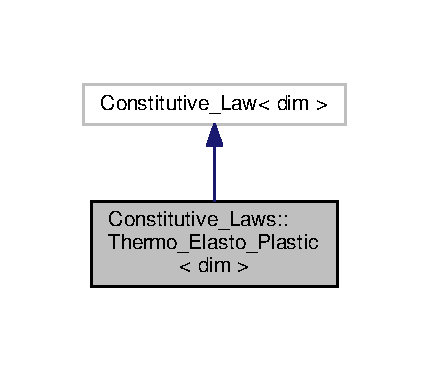
\includegraphics[width=206pt]{classConstitutive__Laws_1_1Thermo__Elasto__Plastic__inherit__graph}
\end{center}
\end{figure}


Collaboration diagram for Constitutive\+\_\+\+Laws\+:\+:Thermo\+\_\+\+Elasto\+\_\+\+Plastic$<$ dim $>$\+:\nopagebreak
\begin{figure}[H]
\begin{center}
\leavevmode
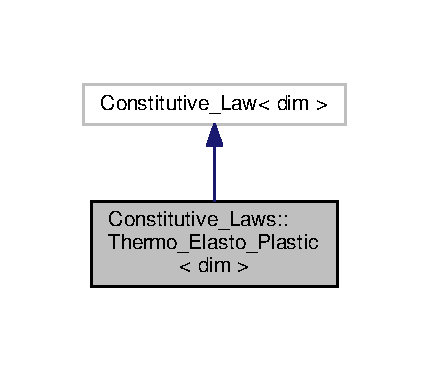
\includegraphics[width=206pt]{classConstitutive__Laws_1_1Thermo__Elasto__Plastic__coll__graph}
\end{center}
\end{figure}
\subsection*{Public Member Functions}
\begin{DoxyCompactItemize}
\item 
\hyperlink{classConstitutive__Laws_1_1Thermo__Elasto__Plastic_a341bfb61aa9e1c3c95a2e423730e397c}{Thermo\+\_\+\+Elasto\+\_\+\+Plastic} (const Parameters\+::\+All\+Parameters$<$ dim $>$ \&prm)
\item 
\hyperlink{classConstitutive__Laws_1_1Thermo__Elasto__Plastic_aee70cb50dfcb1f4d3f3525b870c1f982}{$\sim$\+Thermo\+\_\+\+Elasto\+\_\+\+Plastic} ()=default
\item 
void \hyperlink{classConstitutive__Laws_1_1Thermo__Elasto__Plastic_a1d4b992d9e803ccfbd56d344f9ca7e41}{return\+\_\+stress\+\_\+tangent\+\_\+int\+\_\+variables\+\_\+for\+\_\+small\+\_\+strain} (unsigned int material\+\_\+id, Symmetric\+Tensor$<$ 2, dim $>$ e\+\_\+n1, double alpha\+\_\+n, Symmetric\+Tensor$<$ 2, dim $>$ e\+\_\+n, Symmetric\+Tensor$<$ 2, dim $>$ ep\+\_\+n, Symmetric\+Tensor$<$ 2, dim $>$ eth\+\_\+n, Symmetric\+Tensor$<$ 2, dim $>$ cauchy\+\_\+stress\+\_\+n, double db\+\_\+temperature\+\_\+previous\+\_\+time\+\_\+step, unsigned int int\+\_\+material\+\_\+id\+\_\+previous\+\_\+time\+\_\+step, double db\+\_\+current\+\_\+temperature, double db\+\_\+current\+\_\+time\+\_\+step\+\_\+length, Symmetric\+Tensor$<$ 2, dim $>$ \&cauchy\+\_\+stress, Symmetric\+Tensor$<$ 4, dim $>$ \&elasto\+\_\+plastic\+\_\+tangent\+\_\+ss, Q\+P\+H\+::internal\+\_\+variables\+\_\+incremental$<$ dim $>$ \&updated\+\_\+int\+\_\+variables)
\item 
void \hyperlink{classConstitutive__Laws_1_1Thermo__Elasto__Plastic_a4edcd1aa7b22b47c8522c7bc5f2b211e}{return\+\_\+stress\+\_\+tangent\+\_\+int\+\_\+variables\+\_\+for\+\_\+large\+\_\+strain} (unsigned int material\+\_\+id, Tensor$<$ 2, dim $>$ deformation\+\_\+gradient, double alpha\+\_\+n, Symmetric\+Tensor$<$ 2, dim $>$ e\+\_\+n, Symmetric\+Tensor$<$ 2, dim $>$ ep\+\_\+n, Symmetric\+Tensor$<$ 2, dim $>$ eth\+\_\+n, Symmetric\+Tensor$<$ 2, dim $>$ cauchy\+\_\+stress\+\_\+n, double db\+\_\+temperature\+\_\+previous\+\_\+time\+\_\+step, unsigned int int\+\_\+material\+\_\+id\+\_\+previous\+\_\+time\+\_\+step, double db\+\_\+current\+\_\+temperature, double db\+\_\+current\+\_\+time\+\_\+step\+\_\+length, Symmetric\+Tensor$<$ 2, dim $>$ \&second\+\_\+piola\+\_\+stress, Symmetric\+Tensor$<$ 4, dim $>$ \&elasto\+\_\+plastic\+\_\+tangent, Q\+P\+H\+::internal\+\_\+variables\+\_\+incremental$<$ dim $>$ \&updated\+\_\+int\+\_\+variables)
\end{DoxyCompactItemize}
\subsection*{Private Member Functions}
\begin{DoxyCompactItemize}
\item 
Symmetric\+Tensor$<$ 2, dim $>$ \hyperlink{classConstitutive__Laws_1_1Thermo__Elasto__Plastic_aa0d53eb09b8f27ade4b504ba92c67a73}{return\+\_\+delta\+\_\+e\+\_\+th} (unsigned int material\+\_\+id, unsigned int int\+\_\+material\+\_\+id\+\_\+previous\+\_\+time\+\_\+step, double db\+\_\+temperature\+\_\+previous\+\_\+time\+\_\+step, double db\+\_\+current\+\_\+temperature)
\item 
double \hyperlink{classConstitutive__Laws_1_1Thermo__Elasto__Plastic_a807382a573b93d6c0f2c3aa14ad5b6ac}{return\+\_\+delta\+\_\+lambda} (unsigned int material\+\_\+id, double yield\+\_\+function, double db\+\_\+delta\+\_\+time\+\_\+step, double db\+\_\+current\+\_\+temperature)
\item 
double \hyperlink{classConstitutive__Laws_1_1Thermo__Elasto__Plastic_ae5bc0affd62bea77637f34f641047831}{return\+\_\+yield\+\_\+function} (unsigned int material\+\_\+id, Symmetric\+Tensor$<$ 2, dim $>$ sigma\+\_\+dev\+\_\+trial, double hardening\+\_\+stress\+\_\+\+R\+\_\+trial, double db\+\_\+current\+\_\+temperature)
\item 
double \hyperlink{classConstitutive__Laws_1_1Thermo__Elasto__Plastic_aac67a72f1a65a55f2b155aabb9def3c5}{return\+\_\+hardening\+\_\+stress\+\_\+\+R\+\_\+trial} (unsigned int material\+\_\+id\+\_\+n, unsigned int material\+\_\+id\+\_\+n1, double alpha\+\_\+n, double alpha\+\_\+n1, double db\+\_\+\+T\+\_\+n, double db\+\_\+current\+\_\+temperature)
\item 
Symmetric\+Tensor$<$ 4, dim $>$ \hyperlink{classConstitutive__Laws_1_1Thermo__Elasto__Plastic_ae4b06b02caf03b89ed12254f8e7da816}{return\+\_\+elastic\+\_\+stress\+\_\+strain\+\_\+tensor} (unsigned int material\+\_\+id, double db\+\_\+current\+\_\+temperature)
\item 
Symmetric\+Tensor$<$ 4, dim $>$ \hyperlink{classConstitutive__Laws_1_1Thermo__Elasto__Plastic_a3c565ecee2f2db0511877f2b20302b14}{return\+\_\+elasto\+\_\+plastic\+\_\+stress\+\_\+strain\+\_\+tensor} (unsigned int material\+\_\+id, double sigma\+\_\+dev\+\_\+trial\+\_\+norm, Symmetric\+Tensor$<$ 2, dim $>$ normal, double delta\+\_\+lambda, double db\+\_\+delta\+\_\+timestep, double db\+\_\+current\+\_\+temperature)
\item 
Symmetric\+Tensor$<$ 2, dim $>$ \hyperlink{classConstitutive__Laws_1_1Thermo__Elasto__Plastic_af1cc15583d72208ac71ef846769744ca}{return\+\_\+delta\+\_\+cauchy\+\_\+stress\+\_\+deviator} (unsigned int material\+\_\+id, Symmetric\+Tensor$<$ 2, dim $>$ e\+\_\+delta, Symmetric\+Tensor$<$ 2, dim $>$ ep\+\_\+delta, Symmetric\+Tensor$<$ 2, dim $>$ e\+\_\+n, Symmetric\+Tensor$<$ 2, dim $>$ ep\+\_\+n, double db\+\_\+\+T\+\_\+delta, double db\+\_\+current\+\_\+temperature)
\item 
Symmetric\+Tensor$<$ 2, dim $>$ \hyperlink{classConstitutive__Laws_1_1Thermo__Elasto__Plastic_a5339549a71ccf35f14b23c3286359fa3}{return\+\_\+delta\+\_\+cauchy\+\_\+stress\+\_\+vol} (unsigned int material\+\_\+id, Symmetric\+Tensor$<$ 2, dim $>$ emech\+\_\+delta, Symmetric\+Tensor$<$ 2, dim $>$ emech\+\_\+n, double db\+\_\+\+T\+\_\+delta, double db\+\_\+current\+\_\+temperature)
\end{DoxyCompactItemize}
\subsection*{Private Attributes}
\begin{DoxyCompactItemize}
\item 
Mechanical\+Materials\+::\+Mechanical\+Material$<$ dim $>$ $\ast$ \hyperlink{classConstitutive__Laws_1_1Thermo__Elasto__Plastic_a5a59fd71829d58859a122fe74628a9e4}{ptr\+\_\+mech\+\_\+material}
\item 
const Symmetric\+Tensor$<$ 2, dim $>$ \hyperlink{classConstitutive__Laws_1_1Thermo__Elasto__Plastic_a82407b5024a6bdd7dc424dfa3562acf6}{I} = unit\+\_\+symmetric\+\_\+tensor$<$dim$>$()
\item 
const Symmetric\+Tensor$<$ 4, dim $>$ \hyperlink{classConstitutive__Laws_1_1Thermo__Elasto__Plastic_a3e093ae5b5ef432f1f4fea14148dd8e1}{IxI} = outer\+\_\+product(\hyperlink{classConstitutive__Laws_1_1Thermo__Elasto__Plastic_a82407b5024a6bdd7dc424dfa3562acf6}{I}, \hyperlink{classConstitutive__Laws_1_1Thermo__Elasto__Plastic_a82407b5024a6bdd7dc424dfa3562acf6}{I})
\item 
const Symmetric\+Tensor$<$ 4, dim $>$ \hyperlink{classConstitutive__Laws_1_1Thermo__Elasto__Plastic_a5d88bd28aa5b3e74707ebb49de884755}{deviatoric\+\_\+identity} = deviator\+\_\+tensor$<$dim$>$()
\item 
const unsigned int \hyperlink{classConstitutive__Laws_1_1Thermo__Elasto__Plastic_a4f2bdb1404b0706803da3407ce991667}{material\+\_\+id\+\_\+powder}
\end{DoxyCompactItemize}


\subsection{Constructor \& Destructor Documentation}
\index{Constitutive\+\_\+\+Laws\+::\+Thermo\+\_\+\+Elasto\+\_\+\+Plastic@{Constitutive\+\_\+\+Laws\+::\+Thermo\+\_\+\+Elasto\+\_\+\+Plastic}!Thermo\+\_\+\+Elasto\+\_\+\+Plastic@{Thermo\+\_\+\+Elasto\+\_\+\+Plastic}}
\index{Thermo\+\_\+\+Elasto\+\_\+\+Plastic@{Thermo\+\_\+\+Elasto\+\_\+\+Plastic}!Constitutive\+\_\+\+Laws\+::\+Thermo\+\_\+\+Elasto\+\_\+\+Plastic@{Constitutive\+\_\+\+Laws\+::\+Thermo\+\_\+\+Elasto\+\_\+\+Plastic}}
\subsubsection[{\texorpdfstring{Thermo\+\_\+\+Elasto\+\_\+\+Plastic(const Parameters\+::\+All\+Parameters$<$ dim $>$ \&prm)}{Thermo_Elasto_Plastic(const Parameters::AllParameters< dim > &prm)}}]{\setlength{\rightskip}{0pt plus 5cm}template$<$int dim$>$ {\bf Constitutive\+\_\+\+Laws\+::\+Thermo\+\_\+\+Elasto\+\_\+\+Plastic}$<$ dim $>$\+::{\bf Thermo\+\_\+\+Elasto\+\_\+\+Plastic} (
\begin{DoxyParamCaption}
\item[{const Parameters\+::\+All\+Parameters$<$ dim $>$ \&}]{prm}
\end{DoxyParamCaption}
)}\hypertarget{classConstitutive__Laws_1_1Thermo__Elasto__Plastic_a341bfb61aa9e1c3c95a2e423730e397c}{}\label{classConstitutive__Laws_1_1Thermo__Elasto__Plastic_a341bfb61aa9e1c3c95a2e423730e397c}
\index{Constitutive\+\_\+\+Laws\+::\+Thermo\+\_\+\+Elasto\+\_\+\+Plastic@{Constitutive\+\_\+\+Laws\+::\+Thermo\+\_\+\+Elasto\+\_\+\+Plastic}!````~Thermo\+\_\+\+Elasto\+\_\+\+Plastic@{$\sim$\+Thermo\+\_\+\+Elasto\+\_\+\+Plastic}}
\index{````~Thermo\+\_\+\+Elasto\+\_\+\+Plastic@{$\sim$\+Thermo\+\_\+\+Elasto\+\_\+\+Plastic}!Constitutive\+\_\+\+Laws\+::\+Thermo\+\_\+\+Elasto\+\_\+\+Plastic@{Constitutive\+\_\+\+Laws\+::\+Thermo\+\_\+\+Elasto\+\_\+\+Plastic}}
\subsubsection[{\texorpdfstring{$\sim$\+Thermo\+\_\+\+Elasto\+\_\+\+Plastic()=default}{~Thermo_Elasto_Plastic()=default}}]{\setlength{\rightskip}{0pt plus 5cm}template$<$int dim$>$ {\bf Constitutive\+\_\+\+Laws\+::\+Thermo\+\_\+\+Elasto\+\_\+\+Plastic}$<$ dim $>$\+::$\sim${\bf Thermo\+\_\+\+Elasto\+\_\+\+Plastic} (
\begin{DoxyParamCaption}
{}
\end{DoxyParamCaption}
)\hspace{0.3cm}{\ttfamily [default]}}\hypertarget{classConstitutive__Laws_1_1Thermo__Elasto__Plastic_aee70cb50dfcb1f4d3f3525b870c1f982}{}\label{classConstitutive__Laws_1_1Thermo__Elasto__Plastic_aee70cb50dfcb1f4d3f3525b870c1f982}


\subsection{Member Function Documentation}
\index{Constitutive\+\_\+\+Laws\+::\+Thermo\+\_\+\+Elasto\+\_\+\+Plastic@{Constitutive\+\_\+\+Laws\+::\+Thermo\+\_\+\+Elasto\+\_\+\+Plastic}!return\+\_\+delta\+\_\+cauchy\+\_\+stress\+\_\+deviator@{return\+\_\+delta\+\_\+cauchy\+\_\+stress\+\_\+deviator}}
\index{return\+\_\+delta\+\_\+cauchy\+\_\+stress\+\_\+deviator@{return\+\_\+delta\+\_\+cauchy\+\_\+stress\+\_\+deviator}!Constitutive\+\_\+\+Laws\+::\+Thermo\+\_\+\+Elasto\+\_\+\+Plastic@{Constitutive\+\_\+\+Laws\+::\+Thermo\+\_\+\+Elasto\+\_\+\+Plastic}}
\subsubsection[{\texorpdfstring{return\+\_\+delta\+\_\+cauchy\+\_\+stress\+\_\+deviator(unsigned int material\+\_\+id, Symmetric\+Tensor$<$ 2, dim $>$ e\+\_\+delta, Symmetric\+Tensor$<$ 2, dim $>$ ep\+\_\+delta, Symmetric\+Tensor$<$ 2, dim $>$ e\+\_\+n, Symmetric\+Tensor$<$ 2, dim $>$ ep\+\_\+n, double db\+\_\+\+T\+\_\+delta, double db\+\_\+current\+\_\+temperature)}{return_delta_cauchy_stress_deviator(unsigned int material_id, SymmetricTensor< 2, dim > e_delta, SymmetricTensor< 2, dim > ep_delta, SymmetricTensor< 2, dim > e_n, SymmetricTensor< 2, dim > ep_n, double db_T_delta, double db_current_temperature)}}]{\setlength{\rightskip}{0pt plus 5cm}template$<$int dim$>$ Symmetric\+Tensor$<$ 2, dim $>$ {\bf Constitutive\+\_\+\+Laws\+::\+Thermo\+\_\+\+Elasto\+\_\+\+Plastic}$<$ dim $>$\+::return\+\_\+delta\+\_\+cauchy\+\_\+stress\+\_\+deviator (
\begin{DoxyParamCaption}
\item[{unsigned int}]{material\+\_\+id, }
\item[{Symmetric\+Tensor$<$ 2, dim $>$}]{e\+\_\+delta, }
\item[{Symmetric\+Tensor$<$ 2, dim $>$}]{ep\+\_\+delta, }
\item[{Symmetric\+Tensor$<$ 2, dim $>$}]{e\+\_\+n, }
\item[{Symmetric\+Tensor$<$ 2, dim $>$}]{ep\+\_\+n, }
\item[{double}]{db\+\_\+\+T\+\_\+delta, }
\item[{double}]{db\+\_\+current\+\_\+temperature}
\end{DoxyParamCaption}
)\hspace{0.3cm}{\ttfamily [inline]}, {\ttfamily [private]}}\hypertarget{classConstitutive__Laws_1_1Thermo__Elasto__Plastic_af1cc15583d72208ac71ef846769744ca}{}\label{classConstitutive__Laws_1_1Thermo__Elasto__Plastic_af1cc15583d72208ac71ef846769744ca}


References Constitutive\+\_\+\+Laws\+::\+Thermo\+\_\+\+Elasto\+\_\+\+Plastic$<$ dim $>$\+::ptr\+\_\+mech\+\_\+material.



Referenced by Constitutive\+\_\+\+Laws\+::\+Thermo\+\_\+\+Elasto\+\_\+\+Plastic$<$ dim $>$\+::return\+\_\+stress\+\_\+tangent\+\_\+int\+\_\+variables\+\_\+for\+\_\+small\+\_\+strain().


\begin{DoxyCode}
736                                                                                                            
                      \{
737         SymmetricTensor<2,dim> tmp;
738         \textcolor{keywordtype}{double} db\_shear\_modulus\_at\_current\_temp = \hyperlink{classConstitutive__Laws_1_1Thermo__Elasto__Plastic_a5a59fd71829d58859a122fe74628a9e4}{ptr\_mech\_material}->return\_shear\_modulus(
      material\_id, db\_current\_temperature);
739         \textcolor{keywordtype}{double} db\_dev\_shear\_modulus\_wrt\_temp = \hyperlink{classConstitutive__Laws_1_1Thermo__Elasto__Plastic_a5a59fd71829d58859a122fe74628a9e4}{ptr\_mech\_material}->
      return\_dev\_shear\_modulus\_wrt\_temp(material\_id, db\_current\_temperature);
740 
741         tmp = 2.0 * db\_shear\_modulus\_at\_current\_temp * (deviator(e\_delta) - ep\_delta)
742               + 2.0 * (deviator (e\_n) - ep\_n) * db\_dev\_shear\_modulus\_wrt\_temp * db\_T\_delta;
743 
744         \textcolor{keywordflow}{return} tmp;
745     \}
\end{DoxyCode}
\index{Constitutive\+\_\+\+Laws\+::\+Thermo\+\_\+\+Elasto\+\_\+\+Plastic@{Constitutive\+\_\+\+Laws\+::\+Thermo\+\_\+\+Elasto\+\_\+\+Plastic}!return\+\_\+delta\+\_\+cauchy\+\_\+stress\+\_\+vol@{return\+\_\+delta\+\_\+cauchy\+\_\+stress\+\_\+vol}}
\index{return\+\_\+delta\+\_\+cauchy\+\_\+stress\+\_\+vol@{return\+\_\+delta\+\_\+cauchy\+\_\+stress\+\_\+vol}!Constitutive\+\_\+\+Laws\+::\+Thermo\+\_\+\+Elasto\+\_\+\+Plastic@{Constitutive\+\_\+\+Laws\+::\+Thermo\+\_\+\+Elasto\+\_\+\+Plastic}}
\subsubsection[{\texorpdfstring{return\+\_\+delta\+\_\+cauchy\+\_\+stress\+\_\+vol(unsigned int material\+\_\+id, Symmetric\+Tensor$<$ 2, dim $>$ emech\+\_\+delta, Symmetric\+Tensor$<$ 2, dim $>$ emech\+\_\+n, double db\+\_\+\+T\+\_\+delta, double db\+\_\+current\+\_\+temperature)}{return_delta_cauchy_stress_vol(unsigned int material_id, SymmetricTensor< 2, dim > emech_delta, SymmetricTensor< 2, dim > emech_n, double db_T_delta, double db_current_temperature)}}]{\setlength{\rightskip}{0pt plus 5cm}template$<$int dim$>$ Symmetric\+Tensor$<$ 2, dim $>$ {\bf Constitutive\+\_\+\+Laws\+::\+Thermo\+\_\+\+Elasto\+\_\+\+Plastic}$<$ dim $>$\+::return\+\_\+delta\+\_\+cauchy\+\_\+stress\+\_\+vol (
\begin{DoxyParamCaption}
\item[{unsigned int}]{material\+\_\+id, }
\item[{Symmetric\+Tensor$<$ 2, dim $>$}]{emech\+\_\+delta, }
\item[{Symmetric\+Tensor$<$ 2, dim $>$}]{emech\+\_\+n, }
\item[{double}]{db\+\_\+\+T\+\_\+delta, }
\item[{double}]{db\+\_\+current\+\_\+temperature}
\end{DoxyParamCaption}
)\hspace{0.3cm}{\ttfamily [inline]}, {\ttfamily [private]}}\hypertarget{classConstitutive__Laws_1_1Thermo__Elasto__Plastic_a5339549a71ccf35f14b23c3286359fa3}{}\label{classConstitutive__Laws_1_1Thermo__Elasto__Plastic_a5339549a71ccf35f14b23c3286359fa3}


References Constitutive\+\_\+\+Laws\+::\+Thermo\+\_\+\+Elasto\+\_\+\+Plastic$<$ dim $>$\+::ptr\+\_\+mech\+\_\+material.



Referenced by Constitutive\+\_\+\+Laws\+::\+Thermo\+\_\+\+Elasto\+\_\+\+Plastic$<$ dim $>$\+::return\+\_\+stress\+\_\+tangent\+\_\+int\+\_\+variables\+\_\+for\+\_\+small\+\_\+strain().


\begin{DoxyCode}
752                                                                                                            
                 \{
753         SymmetricTensor<2,dim> tmp;
754         \textcolor{keywordtype}{double} db\_bulk\_modulus\_at\_current\_temp = \hyperlink{classConstitutive__Laws_1_1Thermo__Elasto__Plastic_a5a59fd71829d58859a122fe74628a9e4}{ptr\_mech\_material}->return\_bulk\_modulus(
      material\_id, db\_current\_temperature);
755         \textcolor{keywordtype}{double} db\_dev\_bulk\_modulus\_wrt\_temp = \hyperlink{classConstitutive__Laws_1_1Thermo__Elasto__Plastic_a5a59fd71829d58859a122fe74628a9e4}{ptr\_mech\_material}->
      return\_dev\_bulk\_modolus\_wrt\_temp(material\_id, db\_current\_temperature);
756 
757         tmp= 3.0 * db\_bulk\_modulus\_at\_current\_temp * (emech\_delta - deviator(emech\_delta))
758              + 3.0 * (emech\_n - deviator(emech\_n) ) * db\_dev\_bulk\_modulus\_wrt\_temp * db\_T\_delta;
759 
760         \textcolor{keywordflow}{return} tmp;
761     \}
\end{DoxyCode}
\index{Constitutive\+\_\+\+Laws\+::\+Thermo\+\_\+\+Elasto\+\_\+\+Plastic@{Constitutive\+\_\+\+Laws\+::\+Thermo\+\_\+\+Elasto\+\_\+\+Plastic}!return\+\_\+delta\+\_\+e\+\_\+th@{return\+\_\+delta\+\_\+e\+\_\+th}}
\index{return\+\_\+delta\+\_\+e\+\_\+th@{return\+\_\+delta\+\_\+e\+\_\+th}!Constitutive\+\_\+\+Laws\+::\+Thermo\+\_\+\+Elasto\+\_\+\+Plastic@{Constitutive\+\_\+\+Laws\+::\+Thermo\+\_\+\+Elasto\+\_\+\+Plastic}}
\subsubsection[{\texorpdfstring{return\+\_\+delta\+\_\+e\+\_\+th(unsigned int material\+\_\+id, unsigned int int\+\_\+material\+\_\+id\+\_\+previous\+\_\+time\+\_\+step, double db\+\_\+temperature\+\_\+previous\+\_\+time\+\_\+step, double db\+\_\+current\+\_\+temperature)}{return_delta_e_th(unsigned int material_id, unsigned int int_material_id_previous_time_step, double db_temperature_previous_time_step, double db_current_temperature)}}]{\setlength{\rightskip}{0pt plus 5cm}template$<$int dim$>$ Symmetric\+Tensor$<$ 2, dim $>$ {\bf Constitutive\+\_\+\+Laws\+::\+Thermo\+\_\+\+Elasto\+\_\+\+Plastic}$<$ dim $>$\+::return\+\_\+delta\+\_\+e\+\_\+th (
\begin{DoxyParamCaption}
\item[{unsigned int}]{material\+\_\+id, }
\item[{unsigned int}]{int\+\_\+material\+\_\+id\+\_\+previous\+\_\+time\+\_\+step, }
\item[{double}]{db\+\_\+temperature\+\_\+previous\+\_\+time\+\_\+step, }
\item[{double}]{db\+\_\+current\+\_\+temperature}
\end{DoxyParamCaption}
)\hspace{0.3cm}{\ttfamily [inline]}, {\ttfamily [private]}}\hypertarget{classConstitutive__Laws_1_1Thermo__Elasto__Plastic_aa0d53eb09b8f27ade4b504ba92c67a73}{}\label{classConstitutive__Laws_1_1Thermo__Elasto__Plastic_aa0d53eb09b8f27ade4b504ba92c67a73}


References Constitutive\+\_\+\+Laws\+::\+Thermo\+\_\+\+Elasto\+\_\+\+Plastic$<$ dim $>$\+::I, Constitutive\+\_\+\+Laws\+::\+Thermo\+\_\+\+Elasto\+\_\+\+Plastic$<$ dim $>$\+::material\+\_\+id\+\_\+powder, and Constitutive\+\_\+\+Laws\+::\+Thermo\+\_\+\+Elasto\+\_\+\+Plastic$<$ dim $>$\+::ptr\+\_\+mech\+\_\+material.



Referenced by Constitutive\+\_\+\+Laws\+::\+Thermo\+\_\+\+Elasto\+\_\+\+Plastic$<$ dim $>$\+::return\+\_\+stress\+\_\+tangent\+\_\+int\+\_\+variables\+\_\+for\+\_\+small\+\_\+strain().


\begin{DoxyCode}
642                                                                                  \{
643 
644         SymmetricTensor<2,dim> delta\_eth\_integral;
645         \textcolor{keywordflow}{if}(material\_id == \hyperlink{classConstitutive__Laws_1_1Thermo__Elasto__Plastic_a4f2bdb1404b0706803da3407ce991667}{material\_id\_powder})\{
646             \textcolor{keywordflow}{return} delta\_eth\_integral;
647         \}
648         \textcolor{keywordtype}{double} db\_T\_upper\_bound = db\_current\_temperature;
649         \textcolor{keywordtype}{double} db\_T\_lower\_bound = db\_temperature\_previous\_time\_step;
650         \textcolor{keywordflow}{if}(int\_material\_id\_previous\_time\_step == \hyperlink{classConstitutive__Laws_1_1Thermo__Elasto__Plastic_a4f2bdb1404b0706803da3407ce991667}{material\_id\_powder})\{
651             db\_T\_lower\_bound = \hyperlink{classConstitutive__Laws_1_1Thermo__Elasto__Plastic_a5a59fd71829d58859a122fe74628a9e4}{ptr\_mech\_material}->return\_reference\_temperature();
652         \}
653 
654         \textcolor{keywordtype}{double} integral\_of\_CTE = \hyperlink{classConstitutive__Laws_1_1Thermo__Elasto__Plastic_a5a59fd71829d58859a122fe74628a9e4}{ptr\_mech\_material}->
      return\_expansion\_coefficient\_integral\_form(material\_id,db\_T\_upper\_bound,db\_T\_lower\_bound);
655         delta\_eth\_integral  = integral\_of\_CTE * \hyperlink{classConstitutive__Laws_1_1Thermo__Elasto__Plastic_a82407b5024a6bdd7dc424dfa3562acf6}{I};
656         \textcolor{keywordflow}{return} delta\_eth\_integral;
657     \}
\end{DoxyCode}
\index{Constitutive\+\_\+\+Laws\+::\+Thermo\+\_\+\+Elasto\+\_\+\+Plastic@{Constitutive\+\_\+\+Laws\+::\+Thermo\+\_\+\+Elasto\+\_\+\+Plastic}!return\+\_\+delta\+\_\+lambda@{return\+\_\+delta\+\_\+lambda}}
\index{return\+\_\+delta\+\_\+lambda@{return\+\_\+delta\+\_\+lambda}!Constitutive\+\_\+\+Laws\+::\+Thermo\+\_\+\+Elasto\+\_\+\+Plastic@{Constitutive\+\_\+\+Laws\+::\+Thermo\+\_\+\+Elasto\+\_\+\+Plastic}}
\subsubsection[{\texorpdfstring{return\+\_\+delta\+\_\+lambda(unsigned int material\+\_\+id, double yield\+\_\+function, double db\+\_\+delta\+\_\+time\+\_\+step, double db\+\_\+current\+\_\+temperature)}{return_delta_lambda(unsigned int material_id, double yield_function, double db_delta_time_step, double db_current_temperature)}}]{\setlength{\rightskip}{0pt plus 5cm}template$<$int dim$>$ double {\bf Constitutive\+\_\+\+Laws\+::\+Thermo\+\_\+\+Elasto\+\_\+\+Plastic}$<$ dim $>$\+::return\+\_\+delta\+\_\+lambda (
\begin{DoxyParamCaption}
\item[{unsigned int}]{material\+\_\+id, }
\item[{double}]{yield\+\_\+function, }
\item[{double}]{db\+\_\+delta\+\_\+time\+\_\+step, }
\item[{double}]{db\+\_\+current\+\_\+temperature}
\end{DoxyParamCaption}
)\hspace{0.3cm}{\ttfamily [inline]}, {\ttfamily [private]}}\hypertarget{classConstitutive__Laws_1_1Thermo__Elasto__Plastic_a807382a573b93d6c0f2c3aa14ad5b6ac}{}\label{classConstitutive__Laws_1_1Thermo__Elasto__Plastic_a807382a573b93d6c0f2c3aa14ad5b6ac}


References Constitutive\+\_\+\+Laws\+::\+Thermo\+\_\+\+Elasto\+\_\+\+Plastic$<$ dim $>$\+::ptr\+\_\+mech\+\_\+material.



Referenced by Constitutive\+\_\+\+Laws\+::\+Thermo\+\_\+\+Elasto\+\_\+\+Plastic$<$ dim $>$\+::return\+\_\+stress\+\_\+tangent\+\_\+int\+\_\+variables\+\_\+for\+\_\+small\+\_\+strain().


\begin{DoxyCode}
676                                                                                           \{
677         \textcolor{keywordtype}{double} tmp;
678         \textcolor{keywordtype}{double} db\_shear\_modulus\_at\_current\_temp = \hyperlink{classConstitutive__Laws_1_1Thermo__Elasto__Plastic_a5a59fd71829d58859a122fe74628a9e4}{ptr\_mech\_material}->return\_shear\_modulus(
      material\_id, db\_current\_temperature);
679         \textcolor{keywordtype}{double} db\_hardening\_modulus\_at\_current\_temp = \hyperlink{classConstitutive__Laws_1_1Thermo__Elasto__Plastic_a5a59fd71829d58859a122fe74628a9e4}{ptr\_mech\_material}->
      return\_hardening\_modulus(material\_id, db\_current\_temperature);
680         \textcolor{keywordtype}{double} db\_viscosity\_at\_current\_temp = \hyperlink{classConstitutive__Laws_1_1Thermo__Elasto__Plastic_a5a59fd71829d58859a122fe74628a9e4}{ptr\_mech\_material}->return\_viscosity(
      material\_id, db\_current\_temperature);
681 
682         tmp = yield\_function
683               /
684               (   2.0*db\_shear\_modulus\_at\_current\_temp
685                   + (2.0/3.0) * db\_hardening\_modulus\_at\_current\_temp
686                   + (db\_viscosity\_at\_current\_temp/db\_delta\_time\_step)
687               );
688 
689         \textcolor{keywordflow}{return} tmp;
690     \}
\end{DoxyCode}
\index{Constitutive\+\_\+\+Laws\+::\+Thermo\+\_\+\+Elasto\+\_\+\+Plastic@{Constitutive\+\_\+\+Laws\+::\+Thermo\+\_\+\+Elasto\+\_\+\+Plastic}!return\+\_\+elastic\+\_\+stress\+\_\+strain\+\_\+tensor@{return\+\_\+elastic\+\_\+stress\+\_\+strain\+\_\+tensor}}
\index{return\+\_\+elastic\+\_\+stress\+\_\+strain\+\_\+tensor@{return\+\_\+elastic\+\_\+stress\+\_\+strain\+\_\+tensor}!Constitutive\+\_\+\+Laws\+::\+Thermo\+\_\+\+Elasto\+\_\+\+Plastic@{Constitutive\+\_\+\+Laws\+::\+Thermo\+\_\+\+Elasto\+\_\+\+Plastic}}
\subsubsection[{\texorpdfstring{return\+\_\+elastic\+\_\+stress\+\_\+strain\+\_\+tensor(unsigned int material\+\_\+id, double db\+\_\+current\+\_\+temperature)}{return_elastic_stress_strain_tensor(unsigned int material_id, double db_current_temperature)}}]{\setlength{\rightskip}{0pt plus 5cm}template$<$int dim$>$ Symmetric\+Tensor$<$ 4, dim $>$ {\bf Constitutive\+\_\+\+Laws\+::\+Thermo\+\_\+\+Elasto\+\_\+\+Plastic}$<$ dim $>$\+::return\+\_\+elastic\+\_\+stress\+\_\+strain\+\_\+tensor (
\begin{DoxyParamCaption}
\item[{unsigned int}]{material\+\_\+id, }
\item[{double}]{db\+\_\+current\+\_\+temperature}
\end{DoxyParamCaption}
)\hspace{0.3cm}{\ttfamily [inline]}, {\ttfamily [private]}}\hypertarget{classConstitutive__Laws_1_1Thermo__Elasto__Plastic_ae4b06b02caf03b89ed12254f8e7da816}{}\label{classConstitutive__Laws_1_1Thermo__Elasto__Plastic_ae4b06b02caf03b89ed12254f8e7da816}


References Constitutive\+\_\+\+Laws\+::\+Thermo\+\_\+\+Elasto\+\_\+\+Plastic$<$ dim $>$\+::deviatoric\+\_\+identity, Constitutive\+\_\+\+Laws\+::\+Thermo\+\_\+\+Elasto\+\_\+\+Plastic$<$ dim $>$\+::\+IxI, and Constitutive\+\_\+\+Laws\+::\+Thermo\+\_\+\+Elasto\+\_\+\+Plastic$<$ dim $>$\+::ptr\+\_\+mech\+\_\+material.



Referenced by Constitutive\+\_\+\+Laws\+::\+Thermo\+\_\+\+Elasto\+\_\+\+Plastic$<$ dim $>$\+::return\+\_\+stress\+\_\+tangent\+\_\+int\+\_\+variables\+\_\+for\+\_\+small\+\_\+strain().


\begin{DoxyCode}
717                                                                                                    \{
718         SymmetricTensor<4,dim> tmp;
719 
720         \textcolor{keywordtype}{double} db\_bulk\_modulus\_at\_current\_temp = \hyperlink{classConstitutive__Laws_1_1Thermo__Elasto__Plastic_a5a59fd71829d58859a122fe74628a9e4}{ptr\_mech\_material}->return\_bulk\_modulus(
      material\_id, db\_current\_temperature);
721         \textcolor{keywordtype}{double} db\_shear\_modulus\_at\_current\_temp = \hyperlink{classConstitutive__Laws_1_1Thermo__Elasto__Plastic_a5a59fd71829d58859a122fe74628a9e4}{ptr\_mech\_material}->return\_shear\_modulus(
      material\_id, db\_current\_temperature);
722 
723         tmp =     db\_bulk\_modulus\_at\_current\_temp * \hyperlink{classConstitutive__Laws_1_1Thermo__Elasto__Plastic_a3e093ae5b5ef432f1f4fea14148dd8e1}{IxI}
724                    + 2.0 * db\_shear\_modulus\_at\_current\_temp *\hyperlink{classConstitutive__Laws_1_1Thermo__Elasto__Plastic_a5d88bd28aa5b3e74707ebb49de884755}{deviatoric\_identity};
725 
726         \textcolor{keywordflow}{return} tmp;
727     \}
\end{DoxyCode}
\index{Constitutive\+\_\+\+Laws\+::\+Thermo\+\_\+\+Elasto\+\_\+\+Plastic@{Constitutive\+\_\+\+Laws\+::\+Thermo\+\_\+\+Elasto\+\_\+\+Plastic}!return\+\_\+elasto\+\_\+plastic\+\_\+stress\+\_\+strain\+\_\+tensor@{return\+\_\+elasto\+\_\+plastic\+\_\+stress\+\_\+strain\+\_\+tensor}}
\index{return\+\_\+elasto\+\_\+plastic\+\_\+stress\+\_\+strain\+\_\+tensor@{return\+\_\+elasto\+\_\+plastic\+\_\+stress\+\_\+strain\+\_\+tensor}!Constitutive\+\_\+\+Laws\+::\+Thermo\+\_\+\+Elasto\+\_\+\+Plastic@{Constitutive\+\_\+\+Laws\+::\+Thermo\+\_\+\+Elasto\+\_\+\+Plastic}}
\subsubsection[{\texorpdfstring{return\+\_\+elasto\+\_\+plastic\+\_\+stress\+\_\+strain\+\_\+tensor(unsigned int material\+\_\+id, double sigma\+\_\+dev\+\_\+trial\+\_\+norm, Symmetric\+Tensor$<$ 2, dim $>$ normal, double delta\+\_\+lambda, double db\+\_\+delta\+\_\+timestep, double db\+\_\+current\+\_\+temperature)}{return_elasto_plastic_stress_strain_tensor(unsigned int material_id, double sigma_dev_trial_norm, SymmetricTensor< 2, dim > normal, double delta_lambda, double db_delta_timestep, double db_current_temperature)}}]{\setlength{\rightskip}{0pt plus 5cm}template$<$int dim$>$ Symmetric\+Tensor$<$ 4, dim $>$ {\bf Constitutive\+\_\+\+Laws\+::\+Thermo\+\_\+\+Elasto\+\_\+\+Plastic}$<$ dim $>$\+::return\+\_\+elasto\+\_\+plastic\+\_\+stress\+\_\+strain\+\_\+tensor (
\begin{DoxyParamCaption}
\item[{unsigned int}]{material\+\_\+id, }
\item[{double}]{sigma\+\_\+dev\+\_\+trial\+\_\+norm, }
\item[{Symmetric\+Tensor$<$ 2, dim $>$}]{normal, }
\item[{double}]{delta\+\_\+lambda, }
\item[{double}]{db\+\_\+delta\+\_\+timestep, }
\item[{double}]{db\+\_\+current\+\_\+temperature}
\end{DoxyParamCaption}
)\hspace{0.3cm}{\ttfamily [inline]}, {\ttfamily [private]}}\hypertarget{classConstitutive__Laws_1_1Thermo__Elasto__Plastic_a3c565ecee2f2db0511877f2b20302b14}{}\label{classConstitutive__Laws_1_1Thermo__Elasto__Plastic_a3c565ecee2f2db0511877f2b20302b14}


References Constitutive\+\_\+\+Laws\+::\+Thermo\+\_\+\+Elasto\+\_\+\+Plastic$<$ dim $>$\+::deviatoric\+\_\+identity, Constitutive\+\_\+\+Laws\+::\+Thermo\+\_\+\+Elasto\+\_\+\+Plastic$<$ dim $>$\+::\+IxI, and Constitutive\+\_\+\+Laws\+::\+Thermo\+\_\+\+Elasto\+\_\+\+Plastic$<$ dim $>$\+::ptr\+\_\+mech\+\_\+material.



Referenced by Constitutive\+\_\+\+Laws\+::\+Thermo\+\_\+\+Elasto\+\_\+\+Plastic$<$ dim $>$\+::return\+\_\+stress\+\_\+tangent\+\_\+int\+\_\+variables\+\_\+for\+\_\+small\+\_\+strain().


\begin{DoxyCode}
771     \{
772         SymmetricTensor<4,dim> tmp;
773         \textcolor{keywordtype}{double} db\_bulk\_modulus\_at\_current\_temp = \hyperlink{classConstitutive__Laws_1_1Thermo__Elasto__Plastic_a5a59fd71829d58859a122fe74628a9e4}{ptr\_mech\_material}->return\_bulk\_modulus(
      material\_id, db\_current\_temperature);
774         \textcolor{keywordtype}{double} db\_shear\_modulus\_at\_current\_temp = \hyperlink{classConstitutive__Laws_1_1Thermo__Elasto__Plastic_a5a59fd71829d58859a122fe74628a9e4}{ptr\_mech\_material}->return\_shear\_modulus(
      material\_id, db\_current\_temperature);
775         \textcolor{keywordtype}{double} db\_hardening\_modulus\_at\_current\_temp = \hyperlink{classConstitutive__Laws_1_1Thermo__Elasto__Plastic_a5a59fd71829d58859a122fe74628a9e4}{ptr\_mech\_material}->
      return\_hardening\_modulus(material\_id, db\_current\_temperature);
776         \textcolor{keywordtype}{double} db\_viscosity\_at\_current\_temp = \hyperlink{classConstitutive__Laws_1_1Thermo__Elasto__Plastic_a5a59fd71829d58859a122fe74628a9e4}{ptr\_mech\_material}->return\_viscosity(
      material\_id, db\_current\_temperature);
777 
778         tmp = db\_bulk\_modulus\_at\_current\_temp * \hyperlink{classConstitutive__Laws_1_1Thermo__Elasto__Plastic_a3e093ae5b5ef432f1f4fea14148dd8e1}{IxI}
779               + 2.0  * db\_shear\_modulus\_at\_current\_temp * \hyperlink{classConstitutive__Laws_1_1Thermo__Elasto__Plastic_a5d88bd28aa5b3e74707ebb49de884755}{deviatoric\_identity}
780               - 2.0 * db\_shear\_modulus\_at\_current\_temp *
781                 (
782                         (   (2.0 * db\_shear\_modulus\_at\_current\_temp)
783                             / (2.0 * db\_shear\_modulus\_at\_current\_temp
784                                + (2.0/3.0) * db\_hardening\_modulus\_at\_current\_temp
785                                + (db\_viscosity\_at\_current\_temp / db\_delta\_timestep)
786                             )
787                         ) * outer\_product(normal,normal)
788                         +
789                         (   (2.0 * db\_shear\_modulus\_at\_current\_temp * delta\_lambda )
790                             / sigma\_dev\_trial\_norm
791                         ) * ( \hyperlink{classConstitutive__Laws_1_1Thermo__Elasto__Plastic_a5d88bd28aa5b3e74707ebb49de884755}{deviatoric\_identity} - outer\_product(normal,normal) )
792                 );
793 
794         \textcolor{keywordflow}{return} tmp;
795     \}
\end{DoxyCode}
\index{Constitutive\+\_\+\+Laws\+::\+Thermo\+\_\+\+Elasto\+\_\+\+Plastic@{Constitutive\+\_\+\+Laws\+::\+Thermo\+\_\+\+Elasto\+\_\+\+Plastic}!return\+\_\+hardening\+\_\+stress\+\_\+\+R\+\_\+trial@{return\+\_\+hardening\+\_\+stress\+\_\+\+R\+\_\+trial}}
\index{return\+\_\+hardening\+\_\+stress\+\_\+\+R\+\_\+trial@{return\+\_\+hardening\+\_\+stress\+\_\+\+R\+\_\+trial}!Constitutive\+\_\+\+Laws\+::\+Thermo\+\_\+\+Elasto\+\_\+\+Plastic@{Constitutive\+\_\+\+Laws\+::\+Thermo\+\_\+\+Elasto\+\_\+\+Plastic}}
\subsubsection[{\texorpdfstring{return\+\_\+hardening\+\_\+stress\+\_\+\+R\+\_\+trial(unsigned int material\+\_\+id\+\_\+n, unsigned int material\+\_\+id\+\_\+n1, double alpha\+\_\+n, double alpha\+\_\+n1, double db\+\_\+\+T\+\_\+n, double db\+\_\+current\+\_\+temperature)}{return_hardening_stress_R_trial(unsigned int material_id_n, unsigned int material_id_n1, double alpha_n, double alpha_n1, double db_T_n, double db_current_temperature)}}]{\setlength{\rightskip}{0pt plus 5cm}template$<$int dim$>$ double {\bf Constitutive\+\_\+\+Laws\+::\+Thermo\+\_\+\+Elasto\+\_\+\+Plastic}$<$ dim $>$\+::return\+\_\+hardening\+\_\+stress\+\_\+\+R\+\_\+trial (
\begin{DoxyParamCaption}
\item[{unsigned int}]{material\+\_\+id\+\_\+n, }
\item[{unsigned int}]{material\+\_\+id\+\_\+n1, }
\item[{double}]{alpha\+\_\+n, }
\item[{double}]{alpha\+\_\+n1, }
\item[{double}]{db\+\_\+\+T\+\_\+n, }
\item[{double}]{db\+\_\+current\+\_\+temperature}
\end{DoxyParamCaption}
)\hspace{0.3cm}{\ttfamily [inline]}, {\ttfamily [private]}}\hypertarget{classConstitutive__Laws_1_1Thermo__Elasto__Plastic_aac67a72f1a65a55f2b155aabb9def3c5}{}\label{classConstitutive__Laws_1_1Thermo__Elasto__Plastic_aac67a72f1a65a55f2b155aabb9def3c5}


References Constitutive\+\_\+\+Laws\+::\+Thermo\+\_\+\+Elasto\+\_\+\+Plastic$<$ dim $>$\+::ptr\+\_\+mech\+\_\+material.



Referenced by Constitutive\+\_\+\+Laws\+::\+Thermo\+\_\+\+Elasto\+\_\+\+Plastic$<$ dim $>$\+::return\+\_\+stress\+\_\+tangent\+\_\+int\+\_\+variables\+\_\+for\+\_\+small\+\_\+strain().


\begin{DoxyCode}
698                                                                                                       \{
699         \textcolor{keywordtype}{double} tmp;
700 
701         \textcolor{keywordtype}{double} db\_hardening\_modulus\_at\_current\_temp = \hyperlink{classConstitutive__Laws_1_1Thermo__Elasto__Plastic_a5a59fd71829d58859a122fe74628a9e4}{ptr\_mech\_material}->
      return\_hardening\_modulus(material\_id\_n1, db\_current\_temperature);
702         \textcolor{keywordtype}{double} db\_hardening\_modulus\_at\_T\_n = \hyperlink{classConstitutive__Laws_1_1Thermo__Elasto__Plastic_a5a59fd71829d58859a122fe74628a9e4}{ptr\_mech\_material}->return\_hardening\_modulus(
      material\_id\_n, db\_T\_n);
703         \textcolor{keywordtype}{double} db\_dev\_hardening\_modulus\_wrt\_temp = \hyperlink{classConstitutive__Laws_1_1Thermo__Elasto__Plastic_a5a59fd71829d58859a122fe74628a9e4}{ptr\_mech\_material}->
      return\_dev\_hardening\_modulus\_wrt\_temp(material\_id\_n1, db\_current\_temperature);
704         \textcolor{keywordtype}{double} delta\_alpha = alpha\_n1 - alpha\_n;
705         \textcolor{keywordtype}{double} delta\_temp = db\_current\_temperature - db\_T\_n;
706 
707         tmp = - alpha\_n * db\_hardening\_modulus\_at\_T\_n
708               - (  db\_hardening\_modulus\_at\_current\_temp * delta\_alpha
709                    + db\_dev\_hardening\_modulus\_wrt\_temp * alpha\_n  * delta\_temp );
710 
711         \textcolor{keywordflow}{return} tmp;
712     \}
\end{DoxyCode}
\index{Constitutive\+\_\+\+Laws\+::\+Thermo\+\_\+\+Elasto\+\_\+\+Plastic@{Constitutive\+\_\+\+Laws\+::\+Thermo\+\_\+\+Elasto\+\_\+\+Plastic}!return\+\_\+stress\+\_\+tangent\+\_\+int\+\_\+variables\+\_\+for\+\_\+large\+\_\+strain@{return\+\_\+stress\+\_\+tangent\+\_\+int\+\_\+variables\+\_\+for\+\_\+large\+\_\+strain}}
\index{return\+\_\+stress\+\_\+tangent\+\_\+int\+\_\+variables\+\_\+for\+\_\+large\+\_\+strain@{return\+\_\+stress\+\_\+tangent\+\_\+int\+\_\+variables\+\_\+for\+\_\+large\+\_\+strain}!Constitutive\+\_\+\+Laws\+::\+Thermo\+\_\+\+Elasto\+\_\+\+Plastic@{Constitutive\+\_\+\+Laws\+::\+Thermo\+\_\+\+Elasto\+\_\+\+Plastic}}
\subsubsection[{\texorpdfstring{return\+\_\+stress\+\_\+tangent\+\_\+int\+\_\+variables\+\_\+for\+\_\+large\+\_\+strain(unsigned int material\+\_\+id, Tensor$<$ 2, dim $>$ deformation\+\_\+gradient, double alpha\+\_\+n, Symmetric\+Tensor$<$ 2, dim $>$ e\+\_\+n, Symmetric\+Tensor$<$ 2, dim $>$ ep\+\_\+n, Symmetric\+Tensor$<$ 2, dim $>$ eth\+\_\+n, Symmetric\+Tensor$<$ 2, dim $>$ cauchy\+\_\+stress\+\_\+n, double db\+\_\+temperature\+\_\+previous\+\_\+time\+\_\+step, unsigned int int\+\_\+material\+\_\+id\+\_\+previous\+\_\+time\+\_\+step, double db\+\_\+current\+\_\+temperature, double db\+\_\+current\+\_\+time\+\_\+step\+\_\+length, Symmetric\+Tensor$<$ 2, dim $>$ \&second\+\_\+piola\+\_\+stress, Symmetric\+Tensor$<$ 4, dim $>$ \&elasto\+\_\+plastic\+\_\+tangent, Q\+P\+H\+::internal\+\_\+variables\+\_\+incremental$<$ dim $>$ \&updated\+\_\+int\+\_\+variables)}{return_stress_tangent_int_variables_for_large_strain(unsigned int material_id, Tensor< 2, dim > deformation_gradient, double alpha_n, SymmetricTensor< 2, dim > e_n, SymmetricTensor< 2, dim > ep_n, SymmetricTensor< 2, dim > eth_n, SymmetricTensor< 2, dim > cauchy_stress_n, double db_temperature_previous_time_step, unsigned int int_material_id_previous_time_step, double db_current_temperature, double db_current_time_step_length, SymmetricTensor< 2, dim > &second_piola_stress, SymmetricTensor< 4, dim > &elasto_plastic_tangent, QPH::internal_variables_incremental< dim > &updated_int_variables)}}]{\setlength{\rightskip}{0pt plus 5cm}template$<$int dim$>$ void {\bf Constitutive\+\_\+\+Laws\+::\+Thermo\+\_\+\+Elasto\+\_\+\+Plastic}$<$ dim $>$\+::return\+\_\+stress\+\_\+tangent\+\_\+int\+\_\+variables\+\_\+for\+\_\+large\+\_\+strain (
\begin{DoxyParamCaption}
\item[{unsigned int}]{material\+\_\+id, }
\item[{Tensor$<$ 2, dim $>$}]{deformation\+\_\+gradient, }
\item[{double}]{alpha\+\_\+n, }
\item[{Symmetric\+Tensor$<$ 2, dim $>$}]{e\+\_\+n, }
\item[{Symmetric\+Tensor$<$ 2, dim $>$}]{ep\+\_\+n, }
\item[{Symmetric\+Tensor$<$ 2, dim $>$}]{eth\+\_\+n, }
\item[{Symmetric\+Tensor$<$ 2, dim $>$}]{cauchy\+\_\+stress\+\_\+n, }
\item[{double}]{db\+\_\+temperature\+\_\+previous\+\_\+time\+\_\+step, }
\item[{unsigned int}]{int\+\_\+material\+\_\+id\+\_\+previous\+\_\+time\+\_\+step, }
\item[{double}]{db\+\_\+current\+\_\+temperature, }
\item[{double}]{db\+\_\+current\+\_\+time\+\_\+step\+\_\+length, }
\item[{Symmetric\+Tensor$<$ 2, dim $>$ \&}]{second\+\_\+piola\+\_\+stress, }
\item[{Symmetric\+Tensor$<$ 4, dim $>$ \&}]{elasto\+\_\+plastic\+\_\+tangent, }
\item[{Q\+P\+H\+::internal\+\_\+variables\+\_\+incremental$<$ dim $>$ \&}]{updated\+\_\+int\+\_\+variables}
\end{DoxyParamCaption}
)\hspace{0.3cm}{\ttfamily [inline]}}\hypertarget{classConstitutive__Laws_1_1Thermo__Elasto__Plastic_a4edcd1aa7b22b47c8522c7bc5f2b211e}{}\label{classConstitutive__Laws_1_1Thermo__Elasto__Plastic_a4edcd1aa7b22b47c8522c7bc5f2b211e}


References get\+\_\+tensor\+\_\+operator\+\_\+\+F\+\_\+left(), get\+\_\+tensor\+\_\+operator\+\_\+\+F\+\_\+right(), get\+\_\+tensor\+\_\+operator\+\_\+\+G(), Constitutive\+\_\+\+Laws\+::\+Thermo\+\_\+\+Elasto\+\_\+\+Plastic$<$ dim $>$\+::return\+\_\+stress\+\_\+tangent\+\_\+int\+\_\+variables\+\_\+for\+\_\+small\+\_\+strain(), symmetrize(), and symmetry\+\_\+check().



Referenced by Constitutive\+\_\+\+Laws\+::\+Thermo\+\_\+\+Elasto\+\_\+\+Plastic$<$ dim $>$\+::return\+\_\+stress\+\_\+tangent\+\_\+int\+\_\+variables\+\_\+for\+\_\+small\+\_\+strain().


\begin{DoxyCode}
315     \{
316         \textcolor{keyword}{const} \textcolor{keywordtype}{double} comp\_tolerance = 1e-8;
317 
318         \textcolor{comment}{// Following "Algorithms for computation of stresses and elasticity moduli in terms of Seth–Hill’s
       family of generalized strain tensors" by Miehe&Lambrecht \(\backslash\)n}
319         \textcolor{comment}{// Table I. Algorithm A}
320         \textcolor{comment}{/*}
321 \textcolor{comment}{         * 1. Eigenvalues, eigenvalue bases and diagonal functions:
}
322 \textcolor{comment}{         */}
323 
324         \textcolor{comment}{// Get the symmetric right cauchy green tensor}
325          SymmetricTensor<2, dim> right\_cauchy\_green\_sym = Physics::Elasticity::Kinematics::C(
      deformation\_gradient);
326 
327         \textcolor{comment}{// Compute Eigenvalues, Eigenvectors and Eigenbasis}
328          Vector<double> eigenvalues(dim);
329          std::vector<Tensor<1, dim>> eigenvector(dim);
330          std::vector<SymmetricTensor<2, dim>> eigenbasis(dim);
331          \{
332             \textcolor{comment}{// Get Eigenvalues and Eigenvectors from the deal.ii function \(\backslash\)a eigenvectors(*)}
333             \textcolor{keywordflow}{for} (\textcolor{keywordtype}{unsigned} \textcolor{keywordtype}{int} i = 0; i < dim; ++i) \{
334                 eigenvalues[i] = eigenvectors(right\_cauchy\_green\_sym)[i].first;
335                 eigenvector[i] = eigenvectors(right\_cauchy\_green\_sym)[i].second;
336             \}
337 
338             \textcolor{comment}{// Check if the found eigenvectors are perpendicular to each other}
339             \textcolor{keywordflow}{if} ((std::fabs(eigenvalues(0) - 1) > 1e-10)
340                 && (std::fabs(eigenvalues(1) - 1) > 1e-10)
341                 && (std::fabs(eigenvalues(2) - 1) > 1e-10)) \{
342                 \textcolor{keywordflow}{for} (\textcolor{keywordtype}{unsigned} \textcolor{keywordtype}{int} i = 0; i < dim; ++i) \{
343                     \textcolor{keywordflow}{for} (\textcolor{keywordtype}{unsigned} \textcolor{keywordtype}{int} j = i + 1; j < dim; ++j) \{
344                         AssertThrow( (std::fabs(eigenvector[i] * eigenvector[j]) < 1e-12),
345                                      ExcMessage(\textcolor{stringliteral}{"ln-space<< Eigenvectors are not perpendicular to each
       other."}) );
346                     \}
347                 \}
348             \}
349 
350             \textcolor{comment}{// Compute eigenbasis Ma: eigenbasis = eigenvector \(\backslash\)otimes eigenvector}
351             \textcolor{keywordflow}{for} (\textcolor{keywordtype}{unsigned} \textcolor{keywordtype}{int} i = 0; i < dim; ++i) \{
352                 eigenbasis[i] = \hyperlink{functions_8h_afe83e9509497294b7f662b800b6b91ff}{symmetrize}( outer\_product(eigenvector[i], eigenvector[i]) );
353                 AssertThrow( eigenvalues(i) >= 0.0,
354                              ExcMessage(\textcolor{stringliteral}{"ln-space<< Eigenvalue is negativ. Check update\_qph."}) );
355             \}
356          \}
357 
358         \textcolor{comment}{// Compute diagonal function \(\backslash\)a ea and its first and second derivate \(\backslash\)a da and \(\backslash\)a fa \(\backslash\)n}
359          Vector<double> ea(dim);
360          Vector<double> da(dim);
361          Vector<double> fa(dim);
362          \textcolor{keywordflow}{for} (\textcolor{keywordtype}{unsigned} \textcolor{keywordtype}{int} i = 0; i < dim; ++i)
363          \{
364             ea(i) = 0.5 * std::log( std::abs(eigenvalues(i)) ); \textcolor{comment}{// diagonal function}
365             da(i) = std::pow(eigenvalues(i), -1.0);             \textcolor{comment}{// first derivative of diagonal function ea}
366             fa(i) = -2.0 * std::pow(eigenvalues(i), -2.0);          \textcolor{comment}{// second derivative of diagonal
       function ea}
367             AssertThrow( ea(i) == ea(i),
368                          ExcMessage( \textcolor{stringliteral}{"ln-space<< Ea is nan due to logarithm of negativ eigenvalue. Check
       update\_qph."}) ;
369             AssertThrow( da(i) > 0.0,
370                          ExcMessage( \textcolor{stringliteral}{"ln-space<< First derivative da of diagonal function is "}+
      std::to\_string(da(i))+\textcolor{stringliteral}{" < 0.0 . Check update\_qph."}) );
371          \}
372 
373         \textcolor{comment}{// Compute the Hencky strain}
374          SymmetricTensor<2, dim> hencky\_strain;
375          \textcolor{keywordflow}{for} (\textcolor{keywordtype}{unsigned} \textcolor{keywordtype}{int} a = 0; a < dim; ++a)
376             hencky\_strain += ea(a) * eigenbasis[a];
377 
378         \textcolor{comment}{// Call the small strain material model with the hencky\_strain and history}
379          \textcolor{comment}{// Declare the return arguments}
380           SymmetricTensor<2, dim> stress\_measure\_T\_sym;
381           SymmetricTensor<4,dim> elasto\_plastic\_tangent\_ss;
382 
383          \hyperlink{classConstitutive__Laws_1_1Thermo__Elasto__Plastic_a1d4b992d9e803ccfbd56d344f9ca7e41}{return\_stress\_tangent\_int\_variables\_for\_small\_strain}
384              (
385                 \textcolor{comment}{/*input->*/}
386                 material\_id,
387                 hencky\_strain,
388                 alpha\_n,
389                 e\_n,
390                 ep\_n,
391                 eth\_n,
392                 cauchy\_stress\_n,
393                 db\_temperature\_previous\_time\_step,
394                 int\_material\_id\_previous\_time\_step,
395                 db\_current\_temperature,
396                 db\_current\_time\_step\_length,
397                 \textcolor{comment}{/*output->*/}
398                 stress\_measure\_T\_sym,
399                 elasto\_plastic\_tangent\_ss,
400                 updated\_int\_variables
401             );
402 
403 
404         \textcolor{comment}{/*}
405 \textcolor{comment}{         * 3. Set up coefficients \(\backslash\)a theta, \(\backslash\)a xi and \(\backslash\)a eta (step 2 was bypassed)
}
406 \textcolor{comment}{         */}
407 
408         \textcolor{comment}{// Compute the coefficients based on the eigenvalues, eigenvectors and ea,da,fa}
409          Tensor<2, dim> theta;
410          Tensor<2, dim> xi;
411          \textcolor{keywordtype}{double} eta = 999999999.0;
412 
413         \textcolor{comment}{// For three different eigenvalues \(\backslash\)f$ \(\backslash\)lambda\_a \(\backslash\)neq \(\backslash\)lambda\_b \(\backslash\)neq \(\backslash\)lambda\_c \(\backslash\)f$}
414          \textcolor{keywordflow}{if} (
415                  ( !(std::fabs(eigenvalues(0) - eigenvalues(1)) < comp\_tolerance) )
416                  &&
417                  ( !(std::fabs(eigenvalues(0) - eigenvalues(2)) < comp\_tolerance) )
418                  &&
419                  ( !(std::fabs(eigenvalues(1) - eigenvalues(2)) < comp\_tolerance) )
420              )
421          \{
422             eta = 0.0;
423             \textcolor{keywordflow}{for} (\textcolor{keywordtype}{unsigned} \textcolor{keywordtype}{int} a = 0; a < dim; ++a)
424                 \textcolor{keywordflow}{for} (\textcolor{keywordtype}{unsigned} \textcolor{keywordtype}{int} b = 0; b < dim; ++b)
425                     \textcolor{keywordflow}{if} (a != b)
426                     \{
427                         theta[a][b] = (ea(a) - ea(b))
428                                       / (eigenvalues(a) - eigenvalues(b));
429                         xi[a][b] = (theta[a][b] - 0.5 * da(b))
430                                    / (eigenvalues(a) - eigenvalues(b));
431 
432                         \textcolor{keywordflow}{for} (\textcolor{keywordtype}{unsigned} \textcolor{keywordtype}{int} c = 0; c < dim; ++c)
433                             \textcolor{keywordflow}{if} ((c != a) && (c != b))
434                             \{
435                                 eta +=
436                                         ea(a)
437                                         / (2.0
438                                            * (eigenvalues(a)
439                                               - eigenvalues(b))
440                                            * (eigenvalues(a)
441                                               - eigenvalues(c)));
442                             \}
443                     \}
444          \}
445         \textcolor{comment}{//  For three equal eigenvalues \(\backslash\)f$ \(\backslash\)lambda\_a = \(\backslash\)lambda\_b = \(\backslash\)lambda\_c \(\backslash\)f$}
446          \textcolor{keywordflow}{else} \textcolor{keywordflow}{if} ( (std::fabs(eigenvalues(0) - eigenvalues(1)) < comp\_tolerance)
447                     &&
448                    (std::fabs(eigenvalues(1) - eigenvalues(2)) < comp\_tolerance) )
449          \{
450             eta = 0.0;
451             \textcolor{keywordflow}{for} (\textcolor{keywordtype}{unsigned} \textcolor{keywordtype}{int} a = 0; a < dim; ++a)
452             \{
453                 \textcolor{keywordflow}{for} (\textcolor{keywordtype}{unsigned} \textcolor{keywordtype}{int} b = 0; b < dim; ++b)
454                     \textcolor{keywordflow}{if} (a != b)
455                     \{
456                         theta[a][b] = 0.5 * da(0);
457                         xi[a][b] = (1.0 / 8.0) * fa(0);
458                     \}
459             \}
460             eta = (1.0 / 8.0) * fa(0);
461          \}
462 
463         \textcolor{comment}{// For two equal eigenvalues a and b: \(\backslash\)f$ \(\backslash\)lambda\_a = \(\backslash\)lambda\_b \(\backslash\)neq \(\backslash\)lambda\_c \(\backslash\)f$}
464          \textcolor{keywordflow}{else} \textcolor{keywordflow}{if} ( (std::fabs(eigenvalues(0) - eigenvalues(1)) < comp\_tolerance)
465                    &&
466                    ( !(std::fabs(eigenvalues(1) - eigenvalues(2)) < comp\_tolerance) ) )
467          \{
468             eta = 0.0;
469             \textcolor{keywordflow}{for} (\textcolor{keywordtype}{unsigned} \textcolor{keywordtype}{int} a = 0; a < dim; ++a)
470                 \textcolor{keywordflow}{for} (\textcolor{keywordtype}{unsigned} \textcolor{keywordtype}{int} b = 0; b < dim; ++b)
471                     \textcolor{keywordflow}{if} ((a != b) && ((a == 2) || (b == 2)))
472                     \{
473                         theta[a][b] = (ea(a) - ea(b))
474                                       / (eigenvalues(a) - eigenvalues(b));
475                         xi[a][b] = (theta[a][b] - 0.5 * da(b))
476                                    / (eigenvalues(a) - eigenvalues(b));
477                     \}
478 
479             theta[0][1] = 0.5 * da(0);
480             theta[1][0] = theta[0][1];
481             xi[0][1] = (1.0 / 8.0) * fa(0);
482             xi[1][0] = xi[0][1];
483             eta = xi[2][0];
484          \}
485         \textcolor{comment}{// For two equal eigenvalues a and c: \(\backslash\)f$ \(\backslash\)lambda\_a = \(\backslash\)lambda\_c \(\backslash\)neq \(\backslash\)lambda\_b \(\backslash\)f$}
486          \textcolor{keywordflow}{else} \textcolor{keywordflow}{if} ( (std::fabs(eigenvalues(0) - eigenvalues(2)) < comp\_tolerance)
487                    &&
488                    (!(std::fabs(eigenvalues(1) - eigenvalues(2)) < comp\_tolerance)) )
489          \{
490             eta = 0.0;
491             \textcolor{keywordflow}{for} (\textcolor{keywordtype}{unsigned} \textcolor{keywordtype}{int} a = 0; a < dim; ++a)
492                 \textcolor{keywordflow}{for} (\textcolor{keywordtype}{unsigned} \textcolor{keywordtype}{int} b = 0; b < dim; ++b)
493                     \textcolor{keywordflow}{if} ( (a != b) && ((a == 1) || (b == 1)) )
494                     \{
495                         theta[a][b] = (ea(a) - ea(b))
496                                       / (eigenvalues(a) - eigenvalues(b));
497                         xi[a][b] = (theta[a][b] - 0.5 * da(b))
498                                    / (eigenvalues(a) - eigenvalues(b));
499                     \}
500 
501             theta[0][2] = 0.5 * da(0);
502             theta[2][0] = theta[0][2];
503             xi[0][2] = (1.0 / 8.0) * fa(0);
504             xi[2][0] = xi[0][2];
505             eta = xi[1][0];
506          \}
507         \textcolor{comment}{// For two equal eigenvalues b and c: \(\backslash\)f$ \(\backslash\)lambda\_b = \(\backslash\)lambda\_c \(\backslash\)neq \(\backslash\)lambda\_a \(\backslash\)f$}
508          \textcolor{keywordflow}{else} \textcolor{keywordflow}{if} ( (std::fabs(eigenvalues(1) - eigenvalues(2)) < comp\_tolerance)
509                    &&
510                    (!(std::fabs(eigenvalues(0) - eigenvalues(1)) < comp\_tolerance)) )
511          \{
512             eta = 0.0;
513             \textcolor{keywordflow}{for} (\textcolor{keywordtype}{unsigned} \textcolor{keywordtype}{int} a = 0; a < dim; ++a)
514                 \textcolor{keywordflow}{for} (\textcolor{keywordtype}{unsigned} \textcolor{keywordtype}{int} b = 0; b < dim; ++b)
515                     \textcolor{keywordflow}{if} ( (a != b) && ((a == 0) || (b == 0)) )
516                     \{
517                         theta[a][b] = (ea(a) - ea(b))
518                                       / (eigenvalues(a) - eigenvalues(b));
519                         xi[a][b] = (theta[a][b] - 0.5 * da(b))
520                                    / (eigenvalues(a) - eigenvalues(b));
521                     \}
522 
523             theta[1][2] = 0.5 * da(1);
524             theta[2][1] = theta[1][2];
525             xi[1][2] = (1.0 / 8.0) * fa(1);
526             xi[2][1] = xi[1][2];
527             eta = xi[0][1];
528          \}
529          \textcolor{keywordflow}{else}
530          \{
531             deallog << \textcolor{stringliteral}{"ln-space<< eigenvalues:0: "} << eigenvalues[0] << std::endl;
532             deallog << \textcolor{stringliteral}{"ln-space<< eigenvalues:1: "} << eigenvalues[1] << std::endl;
533             deallog << \textcolor{stringliteral}{"ln-space<< eigenvalues:2: "} << eigenvalues[2] << std::endl;
534             AssertThrow( \textcolor{keyword}{false},
535                          ExcMessage(\textcolor{stringliteral}{"ln-space<< Eigenvalue case not possible, check update\_qph!"}) );
536          \}
537 
538         \textcolor{comment}{// Ensure that \(\backslash\)a eta was initialised in one of the cases}
539          AssertThrow( (eta < 9999999), ExcMessage(\textcolor{stringliteral}{"Eta in update\_qph not initialised"}) );
540 
541 
542         \textcolor{comment}{/*}
543 \textcolor{comment}{         * 4. Lagrangian stresses and elasticity moduli
}
544 \textcolor{comment}{         */}
545 
546         \textcolor{comment}{// Compute projection tensor P}
547          Tensor<4, dim> projection\_tensor\_P;
548          \textcolor{keywordflow}{for} (\textcolor{keywordtype}{unsigned} \textcolor{keywordtype}{int} a = 0; a < dim; ++a)
549          \{
550             projection\_tensor\_P += da(a) * (Tensor<4, dim> ) outer\_product(eigenbasis[a],eigenbasis[a]);
551             \textcolor{keywordflow}{for} (\textcolor{keywordtype}{unsigned} \textcolor{keywordtype}{int} b = 0; b < dim; ++b)
552                 \textcolor{keywordflow}{if} (b != a)
553                     projection\_tensor\_P += theta[a][b] * \hyperlink{functions_8h_a6e649771188b6d625bea6309e77fbd16}{get\_tensor\_operator\_G}(
      eigenbasis[a],eigenbasis[b]);
554          \}
555 
556         \textcolor{comment}{// Check whether the projecton tensor is symmetric and store it into a \(\backslash\)a SymmetricTensor}
557          AssertThrow( \hyperlink{functions_8h_aa37f13547b984cb066e2fcb530b36425}{symmetry\_check}(projection\_tensor\_P), ExcInternalError( \textcolor{stringliteral}{"ln-space<<
       Projection tensor P is not symmetric"}) );
558          SymmetricTensor<4, dim> projection\_tensor\_P\_sym = \hyperlink{functions_8h_afe83e9509497294b7f662b800b6b91ff}{symmetrize}(projection\_tensor\_P);
559 
560         \textcolor{comment}{// Compute the double contraction of T and L}
561          Tensor<4, dim> projection\_tensor\_T\_doublecon\_L;
562          \textcolor{keywordflow}{for} (\textcolor{keywordtype}{unsigned} \textcolor{keywordtype}{int} a = 0; a < dim; ++a)
563          \{
564             projection\_tensor\_T\_doublecon\_L += fa(a)
565                                                * (stress\_measure\_T\_sym * eigenbasis[a])
566                                                * (Tensor<4, dim> ) (outer\_product(eigenbasis[a], eigenbasis
      [a]));
567             \textcolor{keywordflow}{for} (\textcolor{keywordtype}{unsigned} \textcolor{keywordtype}{int} b = 0; b < dim; ++b)
568                 \textcolor{keywordflow}{if} (b != a)
569                 \{
570                     projection\_tensor\_T\_doublecon\_L += 2.0 * xi[a][b]
571                                                        * (
572                                                             
      \hyperlink{functions_8h_acfd8da38df3766246f7bcf0e736ad9f4}{get\_tensor\_operator\_F\_right}(
573                                                                 eigenbasis[a],
574                                                                 eigenbasis[b], eigenbasis[b],
575                                                                 stress\_measure\_T\_sym )
576                                                           + 
      \hyperlink{functions_8h_a6f9435c7728281851248d3537c100e7d}{get\_tensor\_operator\_F\_left}(
577                                                                 eigenbasis[b], eigenbasis[b],
578                                                                 eigenbasis[a],
579                                                                 stress\_measure\_T\_sym )
580                                                           + 
      \hyperlink{functions_8h_acfd8da38df3766246f7bcf0e736ad9f4}{get\_tensor\_operator\_F\_right}(
581                                                                 eigenbasis[b], eigenbasis[a],
582                                                                 eigenbasis[b],
583                                                                 stress\_measure\_T\_sym )
584                                                           + 
      \hyperlink{functions_8h_a6f9435c7728281851248d3537c100e7d}{get\_tensor\_operator\_F\_left}(
585                                                                 eigenbasis[a], eigenbasis[b],
586                                                                 eigenbasis[b],
587                                                                 stress\_measure\_T\_sym )
588                                                           + 
      \hyperlink{functions_8h_acfd8da38df3766246f7bcf0e736ad9f4}{get\_tensor\_operator\_F\_right}(
589                                                                 eigenbasis[b], eigenbasis[b],
590                                                                 eigenbasis[a],
591                                                                 stress\_measure\_T\_sym )
592                                                           + 
      \hyperlink{functions_8h_a6f9435c7728281851248d3537c100e7d}{get\_tensor\_operator\_F\_left}(
593                                                                 eigenbasis[b], eigenbasis[a],
594                                                                 eigenbasis[b],
595                                                                 stress\_measure\_T\_sym )
596                                                            );
597 
598                     \textcolor{keywordflow}{for} (\textcolor{keywordtype}{unsigned} \textcolor{keywordtype}{int} c = 0; c < dim; ++c)
599                         \textcolor{keywordflow}{if} ( (c != a) && (c != b) )
600                         \{
601                             projection\_tensor\_T\_doublecon\_L += 2.0 * eta
602                                                                * (
603                                                                       
      \hyperlink{functions_8h_acfd8da38df3766246f7bcf0e736ad9f4}{get\_tensor\_operator\_F\_right}(
604                                                                         eigenbasis[a], eigenbasis[b],
605                                                                         eigenbasis[c],
606                                                                         stress\_measure\_T\_sym )
607                                                                     + 
      \hyperlink{functions_8h_a6f9435c7728281851248d3537c100e7d}{get\_tensor\_operator\_F\_left}(
608                                                                         eigenbasis[b], eigenbasis[c],
609                                                                         eigenbasis[a],
610                                                                         stress\_measure\_T\_sym )
611                                                                   );
612                         \}
613                 \}
614          \}
615 
616         \textcolor{comment}{// Check whether the tensor is symmetric and store it into a \(\backslash\)a SymmetricTensor}
617          AssertThrow( \hyperlink{functions_8h_aa37f13547b984cb066e2fcb530b36425}{symmetry\_check}(projection\_tensor\_T\_doublecon\_L),
618                       ExcInternalError(\textcolor{stringliteral}{"ln-space<< Projection tensor T:L is not symmetric"}) );
619          SymmetricTensor<4, dim> projection\_tensor\_T\_doublecon\_L\_sym = 
      \hyperlink{functions_8h_afe83e9509497294b7f662b800b6b91ff}{symmetrize}(projection\_tensor\_T\_doublecon\_L);
620 
621         \textcolor{comment}{// Compute the retransformed values}
622          SymmetricTensor<2, dim> second\_piola\_stress\_S;
623          second\_piola\_stress\_S = stress\_measure\_T\_sym
624                                 * projection\_tensor\_P\_sym;
625 
626          elasto\_plastic\_tangent = projection\_tensor\_P\_sym * elasto\_plastic\_tangent\_ss * 
      projection\_tensor\_P\_sym
627                                   + projection\_tensor\_T\_doublecon\_L\_sym;
628          second\_piola\_stress = second\_piola\_stress\_S;
629 
630          updated\_int\_variables.cauchy\_stress\_ls = (second\_piola\_stress * (1 / determinant(
      deformation\_gradient)) );
631     \}
\end{DoxyCode}
\index{Constitutive\+\_\+\+Laws\+::\+Thermo\+\_\+\+Elasto\+\_\+\+Plastic@{Constitutive\+\_\+\+Laws\+::\+Thermo\+\_\+\+Elasto\+\_\+\+Plastic}!return\+\_\+stress\+\_\+tangent\+\_\+int\+\_\+variables\+\_\+for\+\_\+small\+\_\+strain@{return\+\_\+stress\+\_\+tangent\+\_\+int\+\_\+variables\+\_\+for\+\_\+small\+\_\+strain}}
\index{return\+\_\+stress\+\_\+tangent\+\_\+int\+\_\+variables\+\_\+for\+\_\+small\+\_\+strain@{return\+\_\+stress\+\_\+tangent\+\_\+int\+\_\+variables\+\_\+for\+\_\+small\+\_\+strain}!Constitutive\+\_\+\+Laws\+::\+Thermo\+\_\+\+Elasto\+\_\+\+Plastic@{Constitutive\+\_\+\+Laws\+::\+Thermo\+\_\+\+Elasto\+\_\+\+Plastic}}
\subsubsection[{\texorpdfstring{return\+\_\+stress\+\_\+tangent\+\_\+int\+\_\+variables\+\_\+for\+\_\+small\+\_\+strain(unsigned int material\+\_\+id, Symmetric\+Tensor$<$ 2, dim $>$ e\+\_\+n1, double alpha\+\_\+n, Symmetric\+Tensor$<$ 2, dim $>$ e\+\_\+n, Symmetric\+Tensor$<$ 2, dim $>$ ep\+\_\+n, Symmetric\+Tensor$<$ 2, dim $>$ eth\+\_\+n, Symmetric\+Tensor$<$ 2, dim $>$ cauchy\+\_\+stress\+\_\+n, double db\+\_\+temperature\+\_\+previous\+\_\+time\+\_\+step, unsigned int int\+\_\+material\+\_\+id\+\_\+previous\+\_\+time\+\_\+step, double db\+\_\+current\+\_\+temperature, double db\+\_\+current\+\_\+time\+\_\+step\+\_\+length, Symmetric\+Tensor$<$ 2, dim $>$ \&cauchy\+\_\+stress, Symmetric\+Tensor$<$ 4, dim $>$ \&elasto\+\_\+plastic\+\_\+tangent\+\_\+ss, Q\+P\+H\+::internal\+\_\+variables\+\_\+incremental$<$ dim $>$ \&updated\+\_\+int\+\_\+variables)}{return_stress_tangent_int_variables_for_small_strain(unsigned int material_id, SymmetricTensor< 2, dim > e_n1, double alpha_n, SymmetricTensor< 2, dim > e_n, SymmetricTensor< 2, dim > ep_n, SymmetricTensor< 2, dim > eth_n, SymmetricTensor< 2, dim > cauchy_stress_n, double db_temperature_previous_time_step, unsigned int int_material_id_previous_time_step, double db_current_temperature, double db_current_time_step_length, SymmetricTensor< 2, dim > &cauchy_stress, SymmetricTensor< 4, dim > &elasto_plastic_tangent_ss, QPH::internal_variables_incremental< dim > &updated_int_variables)}}]{\setlength{\rightskip}{0pt plus 5cm}template$<$int dim$>$ void {\bf Constitutive\+\_\+\+Laws\+::\+Thermo\+\_\+\+Elasto\+\_\+\+Plastic}$<$ dim $>$\+::return\+\_\+stress\+\_\+tangent\+\_\+int\+\_\+variables\+\_\+for\+\_\+small\+\_\+strain (
\begin{DoxyParamCaption}
\item[{unsigned int}]{material\+\_\+id, }
\item[{Symmetric\+Tensor$<$ 2, dim $>$}]{e\+\_\+n1, }
\item[{double}]{alpha\+\_\+n, }
\item[{Symmetric\+Tensor$<$ 2, dim $>$}]{e\+\_\+n, }
\item[{Symmetric\+Tensor$<$ 2, dim $>$}]{ep\+\_\+n, }
\item[{Symmetric\+Tensor$<$ 2, dim $>$}]{eth\+\_\+n, }
\item[{Symmetric\+Tensor$<$ 2, dim $>$}]{cauchy\+\_\+stress\+\_\+n, }
\item[{double}]{db\+\_\+temperature\+\_\+previous\+\_\+time\+\_\+step, }
\item[{unsigned int}]{int\+\_\+material\+\_\+id\+\_\+previous\+\_\+time\+\_\+step, }
\item[{double}]{db\+\_\+current\+\_\+temperature, }
\item[{double}]{db\+\_\+current\+\_\+time\+\_\+step\+\_\+length, }
\item[{Symmetric\+Tensor$<$ 2, dim $>$ \&}]{cauchy\+\_\+stress, }
\item[{Symmetric\+Tensor$<$ 4, dim $>$ \&}]{elasto\+\_\+plastic\+\_\+tangent\+\_\+ss, }
\item[{Q\+P\+H\+::internal\+\_\+variables\+\_\+incremental$<$ dim $>$ \&}]{updated\+\_\+int\+\_\+variables}
\end{DoxyParamCaption}
)\hspace{0.3cm}{\ttfamily [inline]}}\hypertarget{classConstitutive__Laws_1_1Thermo__Elasto__Plastic_a1d4b992d9e803ccfbd56d344f9ca7e41}{}\label{classConstitutive__Laws_1_1Thermo__Elasto__Plastic_a1d4b992d9e803ccfbd56d344f9ca7e41}


References Constitutive\+\_\+\+Laws\+::\+Thermo\+\_\+\+Elasto\+\_\+\+Plastic$<$ dim $>$\+::ptr\+\_\+mech\+\_\+material, Constitutive\+\_\+\+Laws\+::\+Thermo\+\_\+\+Elasto\+\_\+\+Plastic$<$ dim $>$\+::return\+\_\+delta\+\_\+cauchy\+\_\+stress\+\_\+deviator(), Constitutive\+\_\+\+Laws\+::\+Thermo\+\_\+\+Elasto\+\_\+\+Plastic$<$ dim $>$\+::return\+\_\+delta\+\_\+cauchy\+\_\+stress\+\_\+vol(), Constitutive\+\_\+\+Laws\+::\+Thermo\+\_\+\+Elasto\+\_\+\+Plastic$<$ dim $>$\+::return\+\_\+delta\+\_\+e\+\_\+th(), Constitutive\+\_\+\+Laws\+::\+Thermo\+\_\+\+Elasto\+\_\+\+Plastic$<$ dim $>$\+::return\+\_\+delta\+\_\+lambda(), Constitutive\+\_\+\+Laws\+::\+Thermo\+\_\+\+Elasto\+\_\+\+Plastic$<$ dim $>$\+::return\+\_\+elastic\+\_\+stress\+\_\+strain\+\_\+tensor(), Constitutive\+\_\+\+Laws\+::\+Thermo\+\_\+\+Elasto\+\_\+\+Plastic$<$ dim $>$\+::return\+\_\+elasto\+\_\+plastic\+\_\+stress\+\_\+strain\+\_\+tensor(), Constitutive\+\_\+\+Laws\+::\+Thermo\+\_\+\+Elasto\+\_\+\+Plastic$<$ dim $>$\+::return\+\_\+hardening\+\_\+stress\+\_\+\+R\+\_\+trial(), Constitutive\+\_\+\+Laws\+::\+Thermo\+\_\+\+Elasto\+\_\+\+Plastic$<$ dim $>$\+::return\+\_\+stress\+\_\+tangent\+\_\+int\+\_\+variables\+\_\+for\+\_\+large\+\_\+strain(), and Constitutive\+\_\+\+Laws\+::\+Thermo\+\_\+\+Elasto\+\_\+\+Plastic$<$ dim $>$\+::return\+\_\+yield\+\_\+function().



Referenced by Constitutive\+\_\+\+Laws\+::\+Thermo\+\_\+\+Elasto\+\_\+\+Plastic$<$ dim $>$\+::return\+\_\+stress\+\_\+tangent\+\_\+int\+\_\+variables\+\_\+for\+\_\+large\+\_\+strain().


\begin{DoxyCode}
153                                                                           \{
154 
155         \textcolor{keywordtype}{double} T\_delta = db\_current\_temperature - db\_temperature\_previous\_time\_step;
156         SymmetricTensor<2, dim> ep\_delta;
157         SymmetricTensor<2, dim> eth\_delta = \hyperlink{classConstitutive__Laws_1_1Thermo__Elasto__Plastic_aa0d53eb09b8f27ade4b504ba92c67a73}{return\_delta\_e\_th}(material\_id,
158                                                               int\_material\_id\_previous\_time\_step,
159                                                               db\_temperature\_previous\_time\_step,
160                                                               db\_current\_temperature);
161         SymmetricTensor<2, dim> eth\_n1 = eth\_n + eth\_delta;
162 
163         SymmetricTensor<2, dim> e\_delta = e\_n1 - e\_n;
164         SymmetricTensor<2, dim> sigma\_dev\_trial;
165 
166 
167         \textcolor{keywordflow}{if}(cauchy\_stress\_n.norm() >= 1e-10)\{
168             sigma\_dev\_trial = deviator(cauchy\_stress\_n)
169                               + \hyperlink{classConstitutive__Laws_1_1Thermo__Elasto__Plastic_af1cc15583d72208ac71ef846769744ca}{return\_delta\_cauchy\_stress\_deviator}(
      material\_id,
170                                                                     e\_delta,
171                                                                     ep\_delta,
172                                                                     e\_n,
173                                                                     ep\_n,
174                                                                     T\_delta,
175                                                                     db\_current\_temperature);
176 
177         \}
178         \textcolor{keywordflow}{else}\{
179             sigma\_dev\_trial = \hyperlink{classConstitutive__Laws_1_1Thermo__Elasto__Plastic_af1cc15583d72208ac71ef846769744ca}{return\_delta\_cauchy\_stress\_deviator}(
      material\_id,
180                                                                   e\_delta,
181                                                                   ep\_delta,
182                                                                   e\_n,
183                                                                   ep\_n,
184                                                                   0.0,
185                                                                   db\_current\_temperature);
186         \}
187 
188 
189         SymmetricTensor<2, dim> emech\_n = e\_n - eth\_n \textcolor{comment}{/* - ep\_n */} ; \textcolor{comment}{// the volumetric part of the plastic
       strains is suppost to be 0 so the " - ep\_n" part is not necessary}
190         SymmetricTensor<2, dim> emech\_delta = e\_delta - eth\_delta; \textcolor{comment}{// the volumetric part of the plastic
       strains is suppost to be 0 so the " - ep\_delta" part is not necessary}
191 
192         SymmetricTensor<2, dim> sigma\_vol;
193         \textcolor{keywordflow}{if}(cauchy\_stress\_n.norm() >= 1e-10)\{
194             sigma\_vol = return\_volumetric\_tensor(cauchy\_stress\_n)
195                         + \hyperlink{classConstitutive__Laws_1_1Thermo__Elasto__Plastic_a5339549a71ccf35f14b23c3286359fa3}{return\_delta\_cauchy\_stress\_vol}(material\_id,
196                                                          emech\_delta,
197                                                          emech\_n,
198                                                          T\_delta,
199                                                          db\_current\_temperature);
200         \}
201         \textcolor{keywordflow}{else}\{
202             sigma\_vol = \hyperlink{classConstitutive__Laws_1_1Thermo__Elasto__Plastic_a5339549a71ccf35f14b23c3286359fa3}{return\_delta\_cauchy\_stress\_vol}(material\_id,
203                                                        emech\_delta,
204                                                        emech\_n,
205                                                        0.0,
206                                                        db\_current\_temperature);
207         \}
208 
209         \textcolor{comment}{// compute trial hardening stress}
210         \textcolor{keywordtype}{double} R\_trial = \hyperlink{classConstitutive__Laws_1_1Thermo__Elasto__Plastic_aac67a72f1a65a55f2b155aabb9def3c5}{return\_hardening\_stress\_R\_trial}(
      int\_material\_id\_previous\_time\_step,
211                                                          material\_id,
212                                                          alpha\_n,
213                                                          alpha\_n,
214                                                          db\_temperature\_previous\_time\_step,
215                                                          db\_current\_temperature);
216 
217         \textcolor{comment}{//compute the yield function (von Mises)}
218         \textcolor{keywordtype}{double} phi\_trial = \hyperlink{classConstitutive__Laws_1_1Thermo__Elasto__Plastic_ae5bc0affd62bea77637f34f641047831}{return\_yield\_function}(material\_id,
219                                                  sigma\_dev\_trial,
220                                                  R\_trial,
221                                                  db\_current\_temperature);
222 
223 
224         \textcolor{keywordflow}{if} ( phi\_trial <= 0  \textcolor{comment}{/* elastic case */}   ) \{
225             cauchy\_stress = (sigma\_vol + sigma\_dev\_trial);
226             elasto\_plastic\_tangent\_ss = \hyperlink{classConstitutive__Laws_1_1Thermo__Elasto__Plastic_ae4b06b02caf03b89ed12254f8e7da816}{return\_elastic\_stress\_strain\_tensor}
      (material\_id, db\_current\_temperature);
227 
228             updated\_int\_variables.alpha = alpha\_n;
229             updated\_int\_variables.total\_strain = e\_n1;
230             updated\_int\_variables.plastic\_strain = ep\_n;
231             updated\_int\_variables.thermal\_strain = eth\_n1;
232             updated\_int\_variables.cauchy\_stress = cauchy\_stress;
233             updated\_int\_variables.temperature = db\_current\_temperature;
234             updated\_int\_variables.material\_id = material\_id;
235             updated\_int\_variables.hardening\_stress = R\_trial;
236 
237             \textcolor{keywordflow}{return};
238         \}
239         \textcolor{keywordflow}{else} \{ \textcolor{comment}{/* plastic case */}
240             \textcolor{comment}{//deallog << "PLASTIC CASE " << std::endl;}
241             \textcolor{keywordtype}{double} sigma\_dev\_trial\_norm = sigma\_dev\_trial.norm();
242             SymmetricTensor<2, dim> normal = sigma\_dev\_trial / sigma\_dev\_trial\_norm;
243 
244             \textcolor{keywordtype}{double} delta\_lambda = \hyperlink{classConstitutive__Laws_1_1Thermo__Elasto__Plastic_a807382a573b93d6c0f2c3aa14ad5b6ac}{return\_delta\_lambda}(material\_id, phi\_trial, 
      db\_current\_time\_step\_length, db\_current\_temperature);
245             \textcolor{keywordtype}{double} alpha\_n1 = alpha\_n + delta\_lambda * sqrt(2.0 / 3.0);
246             \textcolor{keywordtype}{double} delta\_R = - delta\_lambda * sqrt(2.0 / 3.0) * 
      \hyperlink{classConstitutive__Laws_1_1Thermo__Elasto__Plastic_a5a59fd71829d58859a122fe74628a9e4}{ptr\_mech\_material}->return\_hardening\_modulus(material\_id, db\_current\_temperature);
247 
248 
249             SymmetricTensor<2, dim> ep\_n1 = ep\_n + delta\_lambda * normal;
250             ep\_delta = ep\_n1 - ep\_n;
251 
252             SymmetricTensor<2, dim> sigma\_dev;
253             \textcolor{keywordflow}{if}(cauchy\_stress\_n.norm()>= 1e-10)\{
254                 sigma\_dev = deviator(cauchy\_stress\_n)
255                             + \hyperlink{classConstitutive__Laws_1_1Thermo__Elasto__Plastic_af1cc15583d72208ac71ef846769744ca}{return\_delta\_cauchy\_stress\_deviator}(
      material\_id,
256                                                                   e\_delta,
257                                                                   ep\_delta,
258                                                                   e\_n,
259                                                                   ep\_n,
260                                                                   T\_delta,
261                                                                   db\_current\_temperature);
262             \}
263             \textcolor{keywordflow}{else}\{
264                 sigma\_dev = \hyperlink{classConstitutive__Laws_1_1Thermo__Elasto__Plastic_af1cc15583d72208ac71ef846769744ca}{return\_delta\_cauchy\_stress\_deviator}(
      material\_id,
265                                                                 e\_delta,
266                                                                 ep\_delta,
267                                                                 e\_n,
268                                                                 ep\_n,
269                                                                 0.0,
270                                                                 db\_current\_temperature);
271             \}
272 
273             cauchy\_stress = sigma\_vol + sigma\_dev;
274             elasto\_plastic\_tangent\_ss = 
      \hyperlink{classConstitutive__Laws_1_1Thermo__Elasto__Plastic_a3c565ecee2f2db0511877f2b20302b14}{return\_elasto\_plastic\_stress\_strain\_tensor}(material\_id,
275                                                                                    sigma\_dev\_trial\_norm,
276                                                                                    normal,
277                                                                                    delta\_lambda,
278                                                                                    
      db\_current\_time\_step\_length,
279                                                                                    db\_current\_temperature);
280 
281             updated\_int\_variables.alpha = alpha\_n1;
282             updated\_int\_variables.total\_strain = e\_n1;
283             updated\_int\_variables.plastic\_strain = ep\_n1;
284             updated\_int\_variables.thermal\_strain = eth\_n1;
285             updated\_int\_variables.cauchy\_stress = cauchy\_stress;
286             updated\_int\_variables.temperature = db\_current\_temperature;
287             updated\_int\_variables.material\_id = material\_id;
288             updated\_int\_variables.hardening\_stress = R\_trial + delta\_R;
289 
290             \textcolor{keywordflow}{return};
291         \}
292     \}
\end{DoxyCode}
\index{Constitutive\+\_\+\+Laws\+::\+Thermo\+\_\+\+Elasto\+\_\+\+Plastic@{Constitutive\+\_\+\+Laws\+::\+Thermo\+\_\+\+Elasto\+\_\+\+Plastic}!return\+\_\+yield\+\_\+function@{return\+\_\+yield\+\_\+function}}
\index{return\+\_\+yield\+\_\+function@{return\+\_\+yield\+\_\+function}!Constitutive\+\_\+\+Laws\+::\+Thermo\+\_\+\+Elasto\+\_\+\+Plastic@{Constitutive\+\_\+\+Laws\+::\+Thermo\+\_\+\+Elasto\+\_\+\+Plastic}}
\subsubsection[{\texorpdfstring{return\+\_\+yield\+\_\+function(unsigned int material\+\_\+id, Symmetric\+Tensor$<$ 2, dim $>$ sigma\+\_\+dev\+\_\+trial, double hardening\+\_\+stress\+\_\+\+R\+\_\+trial, double db\+\_\+current\+\_\+temperature)}{return_yield_function(unsigned int material_id, SymmetricTensor< 2, dim > sigma_dev_trial, double hardening_stress_R_trial, double db_current_temperature)}}]{\setlength{\rightskip}{0pt plus 5cm}template$<$int dim$>$ double {\bf Constitutive\+\_\+\+Laws\+::\+Thermo\+\_\+\+Elasto\+\_\+\+Plastic}$<$ dim $>$\+::return\+\_\+yield\+\_\+function (
\begin{DoxyParamCaption}
\item[{unsigned int}]{material\+\_\+id, }
\item[{Symmetric\+Tensor$<$ 2, dim $>$}]{sigma\+\_\+dev\+\_\+trial, }
\item[{double}]{hardening\+\_\+stress\+\_\+\+R\+\_\+trial, }
\item[{double}]{db\+\_\+current\+\_\+temperature}
\end{DoxyParamCaption}
)\hspace{0.3cm}{\ttfamily [inline]}, {\ttfamily [private]}}\hypertarget{classConstitutive__Laws_1_1Thermo__Elasto__Plastic_ae5bc0affd62bea77637f34f641047831}{}\label{classConstitutive__Laws_1_1Thermo__Elasto__Plastic_ae5bc0affd62bea77637f34f641047831}


References Constitutive\+\_\+\+Laws\+::\+Thermo\+\_\+\+Elasto\+\_\+\+Plastic$<$ dim $>$\+::ptr\+\_\+mech\+\_\+material.



Referenced by Constitutive\+\_\+\+Laws\+::\+Thermo\+\_\+\+Elasto\+\_\+\+Plastic$<$ dim $>$\+::return\+\_\+stress\+\_\+tangent\+\_\+int\+\_\+variables\+\_\+for\+\_\+small\+\_\+strain().


\begin{DoxyCode}
664                                                                                      \{
665         \textcolor{keywordtype}{double} tmp;
666         \textcolor{keywordtype}{double} db\_yield\_stress\_at\_current\_temp = \hyperlink{classConstitutive__Laws_1_1Thermo__Elasto__Plastic_a5a59fd71829d58859a122fe74628a9e4}{ptr\_mech\_material}->return\_yield\_stress(
      material\_id, db\_current\_temperature);
667         tmp = sigma\_dev\_trial.norm() -  sqrt(2.0/3.0) * ( db\_yield\_stress\_at\_current\_temp - 
      hardening\_stress\_R\_trial);
668 
669         \textcolor{keywordflow}{return} tmp;
670     \}
\end{DoxyCode}


\subsection{Member Data Documentation}
\index{Constitutive\+\_\+\+Laws\+::\+Thermo\+\_\+\+Elasto\+\_\+\+Plastic@{Constitutive\+\_\+\+Laws\+::\+Thermo\+\_\+\+Elasto\+\_\+\+Plastic}!deviatoric\+\_\+identity@{deviatoric\+\_\+identity}}
\index{deviatoric\+\_\+identity@{deviatoric\+\_\+identity}!Constitutive\+\_\+\+Laws\+::\+Thermo\+\_\+\+Elasto\+\_\+\+Plastic@{Constitutive\+\_\+\+Laws\+::\+Thermo\+\_\+\+Elasto\+\_\+\+Plastic}}
\subsubsection[{\texorpdfstring{deviatoric\+\_\+identity}{deviatoric_identity}}]{\setlength{\rightskip}{0pt plus 5cm}template$<$int dim$>$ const Symmetric\+Tensor$<$4,dim$>$ {\bf Constitutive\+\_\+\+Laws\+::\+Thermo\+\_\+\+Elasto\+\_\+\+Plastic}$<$ dim $>$\+::deviatoric\+\_\+identity = deviator\+\_\+tensor$<$dim$>$()\hspace{0.3cm}{\ttfamily [private]}}\hypertarget{classConstitutive__Laws_1_1Thermo__Elasto__Plastic_a5d88bd28aa5b3e74707ebb49de884755}{}\label{classConstitutive__Laws_1_1Thermo__Elasto__Plastic_a5d88bd28aa5b3e74707ebb49de884755}


Referenced by Constitutive\+\_\+\+Laws\+::\+Thermo\+\_\+\+Elasto\+\_\+\+Plastic$<$ dim $>$\+::return\+\_\+elastic\+\_\+stress\+\_\+strain\+\_\+tensor(), and Constitutive\+\_\+\+Laws\+::\+Thermo\+\_\+\+Elasto\+\_\+\+Plastic$<$ dim $>$\+::return\+\_\+elasto\+\_\+plastic\+\_\+stress\+\_\+strain\+\_\+tensor().

\index{Constitutive\+\_\+\+Laws\+::\+Thermo\+\_\+\+Elasto\+\_\+\+Plastic@{Constitutive\+\_\+\+Laws\+::\+Thermo\+\_\+\+Elasto\+\_\+\+Plastic}!I@{I}}
\index{I@{I}!Constitutive\+\_\+\+Laws\+::\+Thermo\+\_\+\+Elasto\+\_\+\+Plastic@{Constitutive\+\_\+\+Laws\+::\+Thermo\+\_\+\+Elasto\+\_\+\+Plastic}}
\subsubsection[{\texorpdfstring{I}{I}}]{\setlength{\rightskip}{0pt plus 5cm}template$<$int dim$>$ const Symmetric\+Tensor$<$2,dim$>$ {\bf Constitutive\+\_\+\+Laws\+::\+Thermo\+\_\+\+Elasto\+\_\+\+Plastic}$<$ dim $>$\+::I = unit\+\_\+symmetric\+\_\+tensor$<$dim$>$()\hspace{0.3cm}{\ttfamily [private]}}\hypertarget{classConstitutive__Laws_1_1Thermo__Elasto__Plastic_a82407b5024a6bdd7dc424dfa3562acf6}{}\label{classConstitutive__Laws_1_1Thermo__Elasto__Plastic_a82407b5024a6bdd7dc424dfa3562acf6}


Referenced by Constitutive\+\_\+\+Laws\+::\+Thermo\+\_\+\+Elasto\+\_\+\+Plastic$<$ dim $>$\+::return\+\_\+delta\+\_\+e\+\_\+th().

\index{Constitutive\+\_\+\+Laws\+::\+Thermo\+\_\+\+Elasto\+\_\+\+Plastic@{Constitutive\+\_\+\+Laws\+::\+Thermo\+\_\+\+Elasto\+\_\+\+Plastic}!IxI@{IxI}}
\index{IxI@{IxI}!Constitutive\+\_\+\+Laws\+::\+Thermo\+\_\+\+Elasto\+\_\+\+Plastic@{Constitutive\+\_\+\+Laws\+::\+Thermo\+\_\+\+Elasto\+\_\+\+Plastic}}
\subsubsection[{\texorpdfstring{IxI}{IxI}}]{\setlength{\rightskip}{0pt plus 5cm}template$<$int dim$>$ const Symmetric\+Tensor$<$4,dim$>$ {\bf Constitutive\+\_\+\+Laws\+::\+Thermo\+\_\+\+Elasto\+\_\+\+Plastic}$<$ dim $>$\+::IxI = outer\+\_\+product({\bf I}, {\bf I})\hspace{0.3cm}{\ttfamily [private]}}\hypertarget{classConstitutive__Laws_1_1Thermo__Elasto__Plastic_a3e093ae5b5ef432f1f4fea14148dd8e1}{}\label{classConstitutive__Laws_1_1Thermo__Elasto__Plastic_a3e093ae5b5ef432f1f4fea14148dd8e1}


Referenced by Constitutive\+\_\+\+Laws\+::\+Thermo\+\_\+\+Elasto\+\_\+\+Plastic$<$ dim $>$\+::return\+\_\+elastic\+\_\+stress\+\_\+strain\+\_\+tensor(), and Constitutive\+\_\+\+Laws\+::\+Thermo\+\_\+\+Elasto\+\_\+\+Plastic$<$ dim $>$\+::return\+\_\+elasto\+\_\+plastic\+\_\+stress\+\_\+strain\+\_\+tensor().

\index{Constitutive\+\_\+\+Laws\+::\+Thermo\+\_\+\+Elasto\+\_\+\+Plastic@{Constitutive\+\_\+\+Laws\+::\+Thermo\+\_\+\+Elasto\+\_\+\+Plastic}!material\+\_\+id\+\_\+powder@{material\+\_\+id\+\_\+powder}}
\index{material\+\_\+id\+\_\+powder@{material\+\_\+id\+\_\+powder}!Constitutive\+\_\+\+Laws\+::\+Thermo\+\_\+\+Elasto\+\_\+\+Plastic@{Constitutive\+\_\+\+Laws\+::\+Thermo\+\_\+\+Elasto\+\_\+\+Plastic}}
\subsubsection[{\texorpdfstring{material\+\_\+id\+\_\+powder}{material_id_powder}}]{\setlength{\rightskip}{0pt plus 5cm}template$<$int dim$>$ const unsigned int {\bf Constitutive\+\_\+\+Laws\+::\+Thermo\+\_\+\+Elasto\+\_\+\+Plastic}$<$ dim $>$\+::material\+\_\+id\+\_\+powder\hspace{0.3cm}{\ttfamily [private]}}\hypertarget{classConstitutive__Laws_1_1Thermo__Elasto__Plastic_a4f2bdb1404b0706803da3407ce991667}{}\label{classConstitutive__Laws_1_1Thermo__Elasto__Plastic_a4f2bdb1404b0706803da3407ce991667}


Referenced by Constitutive\+\_\+\+Laws\+::\+Thermo\+\_\+\+Elasto\+\_\+\+Plastic$<$ dim $>$\+::return\+\_\+delta\+\_\+e\+\_\+th().

\index{Constitutive\+\_\+\+Laws\+::\+Thermo\+\_\+\+Elasto\+\_\+\+Plastic@{Constitutive\+\_\+\+Laws\+::\+Thermo\+\_\+\+Elasto\+\_\+\+Plastic}!ptr\+\_\+mech\+\_\+material@{ptr\+\_\+mech\+\_\+material}}
\index{ptr\+\_\+mech\+\_\+material@{ptr\+\_\+mech\+\_\+material}!Constitutive\+\_\+\+Laws\+::\+Thermo\+\_\+\+Elasto\+\_\+\+Plastic@{Constitutive\+\_\+\+Laws\+::\+Thermo\+\_\+\+Elasto\+\_\+\+Plastic}}
\subsubsection[{\texorpdfstring{ptr\+\_\+mech\+\_\+material}{ptr_mech_material}}]{\setlength{\rightskip}{0pt plus 5cm}template$<$int dim$>$ Mechanical\+Materials\+::\+Mechanical\+Material$<$dim$>$$\ast$ {\bf Constitutive\+\_\+\+Laws\+::\+Thermo\+\_\+\+Elasto\+\_\+\+Plastic}$<$ dim $>$\+::ptr\+\_\+mech\+\_\+material\hspace{0.3cm}{\ttfamily [private]}}\hypertarget{classConstitutive__Laws_1_1Thermo__Elasto__Plastic_a5a59fd71829d58859a122fe74628a9e4}{}\label{classConstitutive__Laws_1_1Thermo__Elasto__Plastic_a5a59fd71829d58859a122fe74628a9e4}


Referenced by Constitutive\+\_\+\+Laws\+::\+Thermo\+\_\+\+Elasto\+\_\+\+Plastic$<$ dim $>$\+::return\+\_\+delta\+\_\+cauchy\+\_\+stress\+\_\+deviator(), Constitutive\+\_\+\+Laws\+::\+Thermo\+\_\+\+Elasto\+\_\+\+Plastic$<$ dim $>$\+::return\+\_\+delta\+\_\+cauchy\+\_\+stress\+\_\+vol(), Constitutive\+\_\+\+Laws\+::\+Thermo\+\_\+\+Elasto\+\_\+\+Plastic$<$ dim $>$\+::return\+\_\+delta\+\_\+e\+\_\+th(), Constitutive\+\_\+\+Laws\+::\+Thermo\+\_\+\+Elasto\+\_\+\+Plastic$<$ dim $>$\+::return\+\_\+delta\+\_\+lambda(), Constitutive\+\_\+\+Laws\+::\+Thermo\+\_\+\+Elasto\+\_\+\+Plastic$<$ dim $>$\+::return\+\_\+elastic\+\_\+stress\+\_\+strain\+\_\+tensor(), Constitutive\+\_\+\+Laws\+::\+Thermo\+\_\+\+Elasto\+\_\+\+Plastic$<$ dim $>$\+::return\+\_\+elasto\+\_\+plastic\+\_\+stress\+\_\+strain\+\_\+tensor(), Constitutive\+\_\+\+Laws\+::\+Thermo\+\_\+\+Elasto\+\_\+\+Plastic$<$ dim $>$\+::return\+\_\+hardening\+\_\+stress\+\_\+\+R\+\_\+trial(), Constitutive\+\_\+\+Laws\+::\+Thermo\+\_\+\+Elasto\+\_\+\+Plastic$<$ dim $>$\+::return\+\_\+stress\+\_\+tangent\+\_\+int\+\_\+variables\+\_\+for\+\_\+small\+\_\+strain(), and Constitutive\+\_\+\+Laws\+::\+Thermo\+\_\+\+Elasto\+\_\+\+Plastic$<$ dim $>$\+::return\+\_\+yield\+\_\+function().



The documentation for this class was generated from the following file\+:\begin{DoxyCompactItemize}
\item 
\hyperlink{material_8h}{material.\+h}\end{DoxyCompactItemize}

\chapter{File Documentation}
\hypertarget{functions_8h}{}\section{functions.\+h File Reference}
\label{functions_8h}\index{functions.\+h@{functions.\+h}}
{\ttfamily \#include $<$deal.\+I\+I/base/exceptions.\+h$>$}\\*
{\ttfamily \#include $<$deal.\+I\+I/lac/vector.\+h$>$}\\*
{\ttfamily \#include $<$gsl/gsl\+\_\+integration.\+h$>$}\\*
{\ttfamily \#include $<$gsl/gsl\+\_\+sf\+\_\+gamma.\+h$>$}\\*
{\ttfamily \#include $<$cmath$>$}\\*
{\ttfamily \#include $<$cstdlib$>$}\\*
{\ttfamily \#include $<$numeric$>$}\\*
{\ttfamily \#include $<$stdexcept$>$}\\*
{\ttfamily \#include $<$string$>$}\\*
{\ttfamily \#include $<$utility$>$}\\*
{\ttfamily \#include $<$vector$>$}\\*
Include dependency graph for functions.\+h\+:
\nopagebreak
\begin{figure}[H]
\begin{center}
\leavevmode
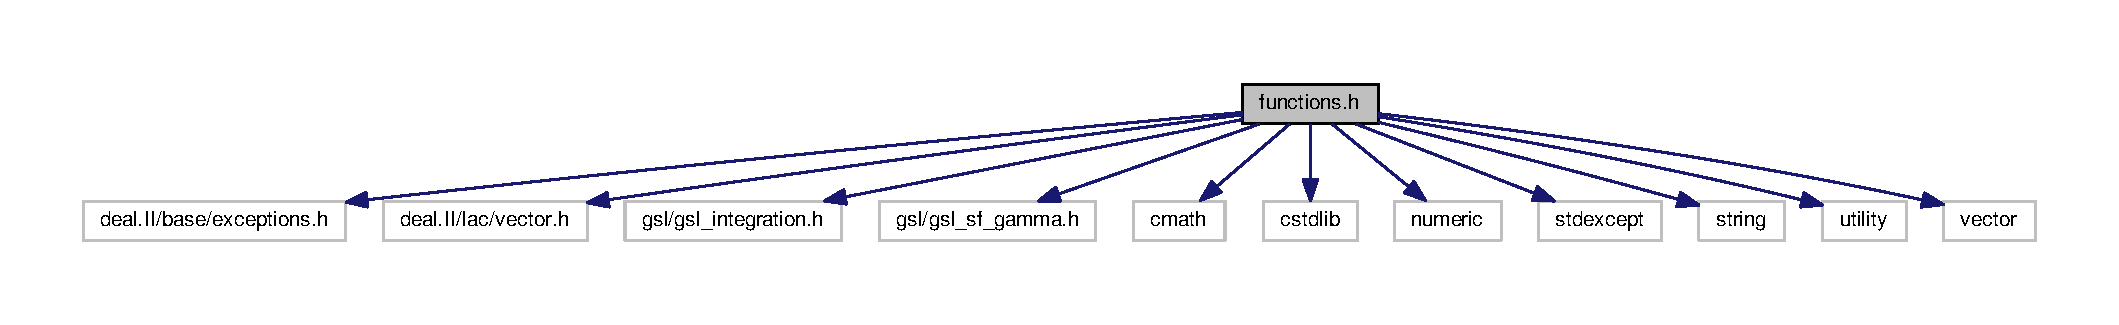
\includegraphics[width=350pt]{functions_8h__incl}
\end{center}
\end{figure}
This graph shows which files directly or indirectly include this file\+:
\nopagebreak
\begin{figure}[H]
\begin{center}
\leavevmode
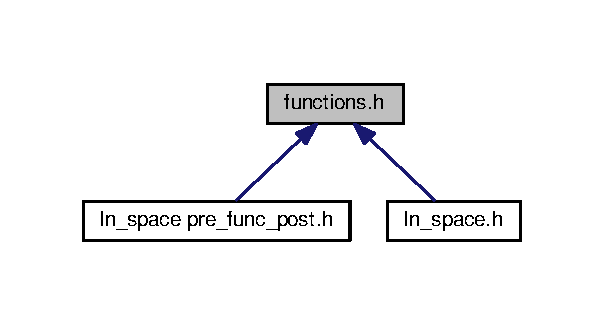
\includegraphics[width=145pt]{functions_8h__dep__incl}
\end{center}
\end{figure}
\subsection*{Macros}
\begin{DoxyCompactItemize}
\item 
\#define \hyperlink{functions_8h_a06d41b26246b319ff9d9b28be162b089}{outer\+\_\+product\+\_\+sym\+\_\+H}
\end{DoxyCompactItemize}
\subsection*{Functions}
\begin{DoxyCompactItemize}
\item 
{\footnotesize template$<$int dim$>$ }\\Tensor$<$ 4, dim $>$ \hyperlink{functions_8h_a6e649771188b6d625bea6309e77fbd16}{get\+\_\+tensor\+\_\+operator\+\_\+G} (const Symmetric\+Tensor$<$ 2, dim $>$ \&Ma, const Symmetric\+Tensor$<$ 2, dim $>$ \&Mb)
\item 
{\footnotesize template$<$int dim$>$ }\\Tensor$<$ 4, dim $>$ \hyperlink{functions_8h_acfd8da38df3766246f7bcf0e736ad9f4}{get\+\_\+tensor\+\_\+operator\+\_\+\+F\+\_\+right} (const Symmetric\+Tensor$<$ 2, dim $>$ \&Ma, const Symmetric\+Tensor$<$ 2, dim $>$ \&Mb, const Symmetric\+Tensor$<$ 2, dim $>$ \&Mc, const Symmetric\+Tensor$<$ 2, dim $>$ \&T)
\item 
{\footnotesize template$<$int dim$>$ }\\Tensor$<$ 4, dim $>$ \hyperlink{functions_8h_a6f9435c7728281851248d3537c100e7d}{get\+\_\+tensor\+\_\+operator\+\_\+\+F\+\_\+left} (const Symmetric\+Tensor$<$ 2, dim $>$ \&Ma, const Symmetric\+Tensor$<$ 2, dim $>$ \&Mb, const Symmetric\+Tensor$<$ 2, dim $>$ \&Mc, const Symmetric\+Tensor$<$ 2, dim $>$ \&T)
\item 
{\footnotesize template$<$int dim$>$ }\\Symmetric\+Tensor$<$ 4, dim $>$ \hyperlink{functions_8h_aa5f33021df9244e49e86b17b15286fa1}{outer\+\_\+product\+\_\+sym} (const Symmetric\+Tensor$<$ 2, dim $>$ \&A, const Symmetric\+Tensor$<$ 2, dim $>$ \&B)
\item 
{\footnotesize template$<$int dim$>$ }\\Symmetric\+Tensor$<$ 4, dim $>$ \hyperlink{functions_8h_a47630aad94c5f95af31f98cec5c0ec9a}{outer\+\_\+product\+\_\+sym} (const Symmetric\+Tensor$<$ 2, dim $>$ \&A)
\item 
{\footnotesize template$<$int dim$>$ }\\Symmetric\+Tensor$<$ 2, dim $>$ \hyperlink{functions_8h_a0ec7a717b44c3db05eb93bc370cca48c}{outer\+\_\+product\+\_\+sym} (const Tensor$<$ 1, dim $>$ \&A)
\item 
{\footnotesize template$<$int dim$>$ }\\bool \hyperlink{functions_8h_aa37f13547b984cb066e2fcb530b36425}{symmetry\+\_\+check} (Tensor$<$ 2, dim $>$ \&tensor)
\item 
{\footnotesize template$<$int dim$>$ }\\bool \hyperlink{functions_8h_adaf42311602a831f5c8c0fffdbb8aa63}{symmetry\+\_\+check} (const Tensor$<$ 4, dim $>$ \&temp)
\item 
{\footnotesize template$<$int dim$>$ }\\Symmetric\+Tensor$<$ 4, dim $>$ \hyperlink{functions_8h_afe83e9509497294b7f662b800b6b91ff}{symmetrize} (const Tensor$<$ 4, dim $>$ \&tensor)
\end{DoxyCompactItemize}


\subsection{Macro Definition Documentation}
\index{functions.\+h@{functions.\+h}!outer\+\_\+product\+\_\+sym\+\_\+H@{outer\+\_\+product\+\_\+sym\+\_\+H}}
\index{outer\+\_\+product\+\_\+sym\+\_\+H@{outer\+\_\+product\+\_\+sym\+\_\+H}!functions.\+h@{functions.\+h}}
\subsubsection[{\texorpdfstring{outer\+\_\+product\+\_\+sym\+\_\+H}{outer_product_sym_H}}]{\setlength{\rightskip}{0pt plus 5cm}\#define outer\+\_\+product\+\_\+sym\+\_\+H}\hypertarget{functions_8h_a06d41b26246b319ff9d9b28be162b089}{}\label{functions_8h_a06d41b26246b319ff9d9b28be162b089}


\subsection{Function Documentation}
\index{functions.\+h@{functions.\+h}!get\+\_\+tensor\+\_\+operator\+\_\+\+F\+\_\+left@{get\+\_\+tensor\+\_\+operator\+\_\+\+F\+\_\+left}}
\index{get\+\_\+tensor\+\_\+operator\+\_\+\+F\+\_\+left@{get\+\_\+tensor\+\_\+operator\+\_\+\+F\+\_\+left}!functions.\+h@{functions.\+h}}
\subsubsection[{\texorpdfstring{get\+\_\+tensor\+\_\+operator\+\_\+\+F\+\_\+left(const Symmetric\+Tensor$<$ 2, dim $>$ \&\+Ma, const Symmetric\+Tensor$<$ 2, dim $>$ \&\+Mb, const Symmetric\+Tensor$<$ 2, dim $>$ \&\+Mc, const Symmetric\+Tensor$<$ 2, dim $>$ \&\+T)}{get_tensor_operator_F_left(const SymmetricTensor< 2, dim > &Ma, const SymmetricTensor< 2, dim > &Mb, const SymmetricTensor< 2, dim > &Mc, const SymmetricTensor< 2, dim > &T)}}]{\setlength{\rightskip}{0pt plus 5cm}template$<$int dim$>$ Tensor$<$4,dim$>$ get\+\_\+tensor\+\_\+operator\+\_\+\+F\+\_\+left (
\begin{DoxyParamCaption}
\item[{const Symmetric\+Tensor$<$ 2, dim $>$ \&}]{Ma, }
\item[{const Symmetric\+Tensor$<$ 2, dim $>$ \&}]{Mb, }
\item[{const Symmetric\+Tensor$<$ 2, dim $>$ \&}]{Mc, }
\item[{const Symmetric\+Tensor$<$ 2, dim $>$ \&}]{T}
\end{DoxyParamCaption}
)}\hypertarget{functions_8h_a6f9435c7728281851248d3537c100e7d}{}\label{functions_8h_a6f9435c7728281851248d3537c100e7d}


Referenced by ln\+\_\+space$<$ dim $>$\+::post\+\_\+ln().


\begin{DoxyCode}
82                                                                          \{
83     Tensor<4,dim> tmp;
84 
85     Tensor<2,dim> temp\_tensor = contract<1,0>((Tensor<2,dim>)T, (Tensor<2,dim>)Mb);
86     Tensor<2,dim> MaTMb = contract<1,0>((Tensor<2,dim>)Ma,temp\_tensor);
87 
88     for(\textcolor{keywordtype}{unsigned} \textcolor{keywordtype}{int} i=0; i<dim; ++i)
89         for(\textcolor{keywordtype}{unsigned} \textcolor{keywordtype}{int} j=0; j<dim; ++j)
90             for(\textcolor{keywordtype}{unsigned} \textcolor{keywordtype}{int} k=0; k<dim; ++k)
91                 for(\textcolor{keywordtype}{unsigned} \textcolor{keywordtype}{int} l=k; l<dim; ++l)
92                 \{
93                     \textcolor{keywordtype}{double} tmp\_scalar = MaTMb[i][k] * Mc[j][l] + MaTMb[i][l] * Mc[j][k];
94                     tmp[i][j][k][l] = tmp\_scalar;
95                     tmp[i][j][l][k] = tmp\_scalar;
96                 \}
97 
98     \textcolor{keywordflow}{return} tmp;
99 \}
\end{DoxyCode}
\index{functions.\+h@{functions.\+h}!get\+\_\+tensor\+\_\+operator\+\_\+\+F\+\_\+right@{get\+\_\+tensor\+\_\+operator\+\_\+\+F\+\_\+right}}
\index{get\+\_\+tensor\+\_\+operator\+\_\+\+F\+\_\+right@{get\+\_\+tensor\+\_\+operator\+\_\+\+F\+\_\+right}!functions.\+h@{functions.\+h}}
\subsubsection[{\texorpdfstring{get\+\_\+tensor\+\_\+operator\+\_\+\+F\+\_\+right(const Symmetric\+Tensor$<$ 2, dim $>$ \&\+Ma, const Symmetric\+Tensor$<$ 2, dim $>$ \&\+Mb, const Symmetric\+Tensor$<$ 2, dim $>$ \&\+Mc, const Symmetric\+Tensor$<$ 2, dim $>$ \&\+T)}{get_tensor_operator_F_right(const SymmetricTensor< 2, dim > &Ma, const SymmetricTensor< 2, dim > &Mb, const SymmetricTensor< 2, dim > &Mc, const SymmetricTensor< 2, dim > &T)}}]{\setlength{\rightskip}{0pt plus 5cm}template$<$int dim$>$ Tensor$<$4,dim$>$ get\+\_\+tensor\+\_\+operator\+\_\+\+F\+\_\+right (
\begin{DoxyParamCaption}
\item[{const Symmetric\+Tensor$<$ 2, dim $>$ \&}]{Ma, }
\item[{const Symmetric\+Tensor$<$ 2, dim $>$ \&}]{Mb, }
\item[{const Symmetric\+Tensor$<$ 2, dim $>$ \&}]{Mc, }
\item[{const Symmetric\+Tensor$<$ 2, dim $>$ \&}]{T}
\end{DoxyParamCaption}
)}\hypertarget{functions_8h_acfd8da38df3766246f7bcf0e736ad9f4}{}\label{functions_8h_acfd8da38df3766246f7bcf0e736ad9f4}


Referenced by ln\+\_\+space$<$ dim $>$\+::post\+\_\+ln().


\begin{DoxyCode}
57 \{
58     Tensor<4,dim> tmp; \textcolor{comment}{// has minor symmetry of indices k,l}
59 
60     Tensor<2,dim> temp\_tensor = contract<1,0>((Tensor<2,dim>)T, (Tensor<2,dim>)Mc);
61     Tensor<2,dim> MbTMc = contract<1,0>((Tensor<2,dim>)Mb,temp\_tensor);
62 
63     for(\textcolor{keywordtype}{unsigned} \textcolor{keywordtype}{int} i=0; i<dim; ++i)
64         for(\textcolor{keywordtype}{unsigned} \textcolor{keywordtype}{int} j=0; j<dim; ++j)
65             for(\textcolor{keywordtype}{unsigned} \textcolor{keywordtype}{int} k=0; k<dim; ++k)
66                 for(\textcolor{keywordtype}{unsigned} \textcolor{keywordtype}{int} l=k; l<dim; ++l)
67                 \{
68                     \textcolor{keywordtype}{double} tmp\_scalar = Ma[i][k] * MbTMc[j][l] + Ma[i][l] * MbTMc[j][k];
69                     tmp[i][j][k][l] = tmp\_scalar;
70                     tmp[i][j][l][k] = tmp\_scalar;
71                 \}
72 
73     \textcolor{keywordflow}{return} tmp;
74 \}
\end{DoxyCode}
\index{functions.\+h@{functions.\+h}!get\+\_\+tensor\+\_\+operator\+\_\+G@{get\+\_\+tensor\+\_\+operator\+\_\+G}}
\index{get\+\_\+tensor\+\_\+operator\+\_\+G@{get\+\_\+tensor\+\_\+operator\+\_\+G}!functions.\+h@{functions.\+h}}
\subsubsection[{\texorpdfstring{get\+\_\+tensor\+\_\+operator\+\_\+\+G(const Symmetric\+Tensor$<$ 2, dim $>$ \&\+Ma, const Symmetric\+Tensor$<$ 2, dim $>$ \&\+Mb)}{get_tensor_operator_G(const SymmetricTensor< 2, dim > &Ma, const SymmetricTensor< 2, dim > &Mb)}}]{\setlength{\rightskip}{0pt plus 5cm}template$<$int dim$>$ Tensor$<$4,dim$>$ get\+\_\+tensor\+\_\+operator\+\_\+G (
\begin{DoxyParamCaption}
\item[{const Symmetric\+Tensor$<$ 2, dim $>$ \&}]{Ma, }
\item[{const Symmetric\+Tensor$<$ 2, dim $>$ \&}]{Mb}
\end{DoxyParamCaption}
)}\hypertarget{functions_8h_a6e649771188b6d625bea6309e77fbd16}{}\label{functions_8h_a6e649771188b6d625bea6309e77fbd16}


Referenced by ln\+\_\+space$<$ dim $>$\+::post\+\_\+ln().


\begin{DoxyCode}
34 \{
35     Tensor<4,dim> tmp; \textcolor{comment}{// has minor symmetry of indices k,l}
36 
37     \textcolor{keywordflow}{for}(\textcolor{keywordtype}{unsigned} \textcolor{keywordtype}{int} i=0; i<dim; ++i)
38         \textcolor{keywordflow}{for}(\textcolor{keywordtype}{unsigned} \textcolor{keywordtype}{int} j=0; j<dim; ++j)
39             \textcolor{keywordflow}{for}(\textcolor{keywordtype}{unsigned} \textcolor{keywordtype}{int} k=0; k<dim; ++k)
40                 \textcolor{keywordflow}{for}(\textcolor{keywordtype}{unsigned} \textcolor{keywordtype}{int} l=k; l<dim; ++l)
41                 \{
42                     \textcolor{keywordtype}{double} tmp\_scalar = Ma[i][k] * Mb[j][l] + Ma[i][l] * Mb[j][k];
43                     tmp[i][j][k][l] = tmp\_scalar;
44                     tmp[i][j][l][k] = tmp\_scalar;
45                 \}
46 
47     \textcolor{keywordflow}{return} tmp;
48 \}
\end{DoxyCode}
\index{functions.\+h@{functions.\+h}!outer\+\_\+product\+\_\+sym@{outer\+\_\+product\+\_\+sym}}
\index{outer\+\_\+product\+\_\+sym@{outer\+\_\+product\+\_\+sym}!functions.\+h@{functions.\+h}}
\subsubsection[{\texorpdfstring{outer\+\_\+product\+\_\+sym(const Symmetric\+Tensor$<$ 2, dim $>$ \&\+A, const Symmetric\+Tensor$<$ 2, dim $>$ \&\+B)}{outer_product_sym(const SymmetricTensor< 2, dim > &A, const SymmetricTensor< 2, dim > &B)}}]{\setlength{\rightskip}{0pt plus 5cm}template$<$int dim$>$ Symmetric\+Tensor$<$4,dim$>$ outer\+\_\+product\+\_\+sym (
\begin{DoxyParamCaption}
\item[{const Symmetric\+Tensor$<$ 2, dim $>$ \&}]{A, }
\item[{const Symmetric\+Tensor$<$ 2, dim $>$ \&}]{B}
\end{DoxyParamCaption}
)}\hypertarget{functions_8h_aa5f33021df9244e49e86b17b15286fa1}{}\label{functions_8h_aa5f33021df9244e49e86b17b15286fa1}


Referenced by ln\+\_\+space$<$ dim $>$\+::plastic\+\_\+right\+\_\+cauchy\+\_\+green\+\_\+\+A\+S(), ln\+\_\+space$<$ dim $>$\+::post\+\_\+ln(), and ln\+\_\+space$<$ dim $>$\+::pre\+\_\+ln().


\begin{DoxyCode}
111 \{
112     SymmetricTensor<4,dim> D;
113     \textcolor{comment}{// Special nested for-loop to access only non-symmetric entries of 4th order sym. tensor}
114     \textcolor{comment}{// ToDo: still not optimal element 1112 and 1211 are both accessed}
115     \textcolor{keywordflow}{for} ( \textcolor{keywordtype}{unsigned} \textcolor{keywordtype}{int} i=0; i<dim; ++i )
116         \textcolor{keywordflow}{for} ( \textcolor{keywordtype}{unsigned} \textcolor{keywordtype}{int} j=i; j<dim; ++j )
117             \textcolor{keywordflow}{for} ( \textcolor{keywordtype}{unsigned} \textcolor{keywordtype}{int} k=i; k<dim; ++k )
118                 \textcolor{keywordflow}{for} ( \textcolor{keywordtype}{unsigned} \textcolor{keywordtype}{int} l=k; l<dim; ++l )
119                 \{
120                     \textcolor{keywordtype}{double} tmp = A[i][j] * B[k][l] + B[i][j] * A[k][l];
121                     D[i][j][k][l] = tmp;
122                     D[k][l][i][j] = tmp;
123                 \}
124     \textcolor{keywordflow}{return} D;
125 \}
\end{DoxyCode}
\index{functions.\+h@{functions.\+h}!outer\+\_\+product\+\_\+sym@{outer\+\_\+product\+\_\+sym}}
\index{outer\+\_\+product\+\_\+sym@{outer\+\_\+product\+\_\+sym}!functions.\+h@{functions.\+h}}
\subsubsection[{\texorpdfstring{outer\+\_\+product\+\_\+sym(const Symmetric\+Tensor$<$ 2, dim $>$ \&\+A)}{outer_product_sym(const SymmetricTensor< 2, dim > &A)}}]{\setlength{\rightskip}{0pt plus 5cm}template$<$int dim$>$ Symmetric\+Tensor$<$4,dim$>$ outer\+\_\+product\+\_\+sym (
\begin{DoxyParamCaption}
\item[{const Symmetric\+Tensor$<$ 2, dim $>$ \&}]{A}
\end{DoxyParamCaption}
)}\hypertarget{functions_8h_a47630aad94c5f95af31f98cec5c0ec9a}{}\label{functions_8h_a47630aad94c5f95af31f98cec5c0ec9a}

\begin{DoxyCode}
128 \{
129     SymmetricTensor<4,dim> D;
130     \textcolor{comment}{// Special nested for-loop to access only non-symmetric entries of 4th order sym. tensor}
131     \textcolor{comment}{// ToDo: still not optimal element 1112 and 1211 are both accessed}
132     \textcolor{keywordflow}{for} ( \textcolor{keywordtype}{unsigned} \textcolor{keywordtype}{int} i=0; i<dim; ++i )
133         \textcolor{keywordflow}{for} ( \textcolor{keywordtype}{unsigned} \textcolor{keywordtype}{int} j=i; j<dim; ++j )
134             \textcolor{keywordflow}{for} ( \textcolor{keywordtype}{unsigned} \textcolor{keywordtype}{int} k=i; k<dim; ++k )
135                 \textcolor{keywordflow}{for} ( \textcolor{keywordtype}{unsigned} \textcolor{keywordtype}{int} l=k; l<dim; ++l )
136                 \{
137                     \textcolor{keywordtype}{double} tmp = A[i][j] * A[k][l];
138                     D[i][j][k][l] = tmp;
139                     D[k][l][i][j] = tmp;
140                 \}
141     \textcolor{keywordflow}{return} D;
142 \}
\end{DoxyCode}
\index{functions.\+h@{functions.\+h}!outer\+\_\+product\+\_\+sym@{outer\+\_\+product\+\_\+sym}}
\index{outer\+\_\+product\+\_\+sym@{outer\+\_\+product\+\_\+sym}!functions.\+h@{functions.\+h}}
\subsubsection[{\texorpdfstring{outer\+\_\+product\+\_\+sym(const Tensor$<$ 1, dim $>$ \&\+A)}{outer_product_sym(const Tensor< 1, dim > &A)}}]{\setlength{\rightskip}{0pt plus 5cm}template$<$int dim$>$ Symmetric\+Tensor$<$2,dim$>$ outer\+\_\+product\+\_\+sym (
\begin{DoxyParamCaption}
\item[{const Tensor$<$ 1, dim $>$ \&}]{A}
\end{DoxyParamCaption}
)}\hypertarget{functions_8h_a0ec7a717b44c3db05eb93bc370cca48c}{}\label{functions_8h_a0ec7a717b44c3db05eb93bc370cca48c}

\begin{DoxyCode}
145 \{
146     SymmetricTensor<2,dim> D;
147     \textcolor{comment}{// Special nested for-loop to access only non-symmetric entries of 4th order sym. tensor}
148     \textcolor{comment}{// ToDo: still not optimal element 1112 and 1211 are both accessed}
149     \textcolor{keywordflow}{for} ( \textcolor{keywordtype}{unsigned} \textcolor{keywordtype}{int} i=0; i<dim; ++i )
150         \textcolor{keywordflow}{for} ( \textcolor{keywordtype}{unsigned} \textcolor{keywordtype}{int} j=i; j<dim; ++j )
151             D[i][j] = A[i] * A[j];
152 
153     \textcolor{keywordflow}{return} D;
154 \}
\end{DoxyCode}
\index{functions.\+h@{functions.\+h}!symmetrize@{symmetrize}}
\index{symmetrize@{symmetrize}!functions.\+h@{functions.\+h}}
\subsubsection[{\texorpdfstring{symmetrize(const Tensor$<$ 4, dim $>$ \&tensor)}{symmetrize(const Tensor< 4, dim > &tensor)}}]{\setlength{\rightskip}{0pt plus 5cm}template$<$int dim$>$ Symmetric\+Tensor$<$4,dim$>$ symmetrize (
\begin{DoxyParamCaption}
\item[{const Tensor$<$ 4, dim $>$ \&}]{tensor}
\end{DoxyParamCaption}
)}\hypertarget{functions_8h_afe83e9509497294b7f662b800b6b91ff}{}\label{functions_8h_afe83e9509497294b7f662b800b6b91ff}


References symmetry\+\_\+check().



Referenced by ln\+\_\+space$<$ dim $>$\+::post\+\_\+ln(), and ln\+\_\+space$<$ dim $>$\+::pre\+\_\+ln().


\begin{DoxyCode}
209                                                               \{
210     SymmetricTensor<4,dim> sym\_tensor;
211     Assert(\hyperlink{functions_8h_aa37f13547b984cb066e2fcb530b36425}{symmetry\_check}(tensor), ExcMessage(\textcolor{stringliteral}{"Tensor to symmetrize is not symmetric!"}));
212 
213     Tensor<4,dim> temp\_tensor;
214     \textcolor{keywordflow}{for}(\textcolor{keywordtype}{unsigned} \textcolor{keywordtype}{int} i=0; i<dim; ++i)
215         \textcolor{keywordflow}{for}(\textcolor{keywordtype}{unsigned} \textcolor{keywordtype}{int} j=0; j<dim; ++j)
216             \textcolor{keywordflow}{for}(\textcolor{keywordtype}{unsigned} \textcolor{keywordtype}{int} k=0; k<dim; ++k)
217                 \textcolor{keywordflow}{for}(\textcolor{keywordtype}{unsigned} \textcolor{keywordtype}{int} l=0; l<dim; ++l)
218                     temp\_tensor[i][j][k][l] = (tensor[i][j][k][l]+tensor[j][i][k][l]+tensor[i][j][l][k]) / 
      3.0;
219 
220     \textcolor{keywordflow}{for}(\textcolor{keywordtype}{unsigned} \textcolor{keywordtype}{int} i=0; i<dim; ++i)
221         \textcolor{keywordflow}{for}(\textcolor{keywordtype}{unsigned} \textcolor{keywordtype}{int} j=i; j<dim; ++j)
222             \textcolor{keywordflow}{for}(\textcolor{keywordtype}{unsigned} \textcolor{keywordtype}{int} k=0; k<dim; ++k)
223                 \textcolor{keywordflow}{for}(\textcolor{keywordtype}{unsigned} \textcolor{keywordtype}{int} l=k; l<dim; ++l)
224                     sym\_tensor[i][j][k][l] = temp\_tensor[i][j][k][l];
225 \textcolor{comment}{//                    sym\_tensor[i][j][k][l] = tensor[i][j][k][l];}
226 
227     \textcolor{keywordflow}{return} sym\_tensor;
228 \}
\end{DoxyCode}
\index{functions.\+h@{functions.\+h}!symmetry\+\_\+check@{symmetry\+\_\+check}}
\index{symmetry\+\_\+check@{symmetry\+\_\+check}!functions.\+h@{functions.\+h}}
\subsubsection[{\texorpdfstring{symmetry\+\_\+check(\+Tensor$<$ 2, dim $>$ \&tensor)}{symmetry_check(Tensor< 2, dim > &tensor)}}]{\setlength{\rightskip}{0pt plus 5cm}template$<$int dim$>$ bool symmetry\+\_\+check (
\begin{DoxyParamCaption}
\item[{Tensor$<$ 2, dim $>$ \&}]{tensor}
\end{DoxyParamCaption}
)}\hypertarget{functions_8h_aa37f13547b984cb066e2fcb530b36425}{}\label{functions_8h_aa37f13547b984cb066e2fcb530b36425}


Referenced by ln\+\_\+space$<$ dim $>$\+::post\+\_\+ln(), and symmetrize().


\begin{DoxyCode}
164 \{
165     \textcolor{keywordflow}{for} ( \textcolor{keywordtype}{unsigned} \textcolor{keywordtype}{int} i=0; i<dim; i++ )
166         \textcolor{keywordflow}{for} ( \textcolor{keywordtype}{unsigned} \textcolor{keywordtype}{int} j=0; j<dim; j++ )
167             \textcolor{keywordflow}{if} ( i!=j && ( std::abs(tensor[i][j] - tensor[j][i])>1e-12 ) )
168                 \textcolor{keywordflow}{return} \textcolor{keyword}{false};
169 
170     \textcolor{keywordflow}{return} \textcolor{keyword}{true};
171 \}
\end{DoxyCode}
\index{functions.\+h@{functions.\+h}!symmetry\+\_\+check@{symmetry\+\_\+check}}
\index{symmetry\+\_\+check@{symmetry\+\_\+check}!functions.\+h@{functions.\+h}}
\subsubsection[{\texorpdfstring{symmetry\+\_\+check(const Tensor$<$ 4, dim $>$ \&temp)}{symmetry_check(const Tensor< 4, dim > &temp)}}]{\setlength{\rightskip}{0pt plus 5cm}template$<$int dim$>$ bool symmetry\+\_\+check (
\begin{DoxyParamCaption}
\item[{const Tensor$<$ 4, dim $>$ \&}]{temp}
\end{DoxyParamCaption}
)}\hypertarget{functions_8h_adaf42311602a831f5c8c0fffdbb8aa63}{}\label{functions_8h_adaf42311602a831f5c8c0fffdbb8aa63}

\begin{DoxyCode}
173                                               \{
174     \textcolor{keywordflow}{for}(\textcolor{keywordtype}{unsigned} \textcolor{keywordtype}{int} i=0; i<dim; ++i)\{
175         \textcolor{keywordflow}{for}(\textcolor{keywordtype}{unsigned} \textcolor{keywordtype}{int} j=0; j<dim; ++j)\{
176             \textcolor{keywordflow}{for}(\textcolor{keywordtype}{unsigned} \textcolor{keywordtype}{int} k=0; k<dim; ++k)\{
177                 \textcolor{keywordflow}{for}(\textcolor{keywordtype}{unsigned} \textcolor{keywordtype}{int} l=0; l<dim; ++l)\{
178                     \textcolor{comment}{// absolute difference check}
179                     \textcolor{keywordflow}{if}(    ( fabs(temp[i][j][k][l] - temp[j][i][k][l]) > 1e-6 )
180                             ||
181                           ( fabs(temp[i][j][k][l] - temp[i][j][l][k]) > 1e-6 ) )
182                     \{
183                         \textcolor{comment}{// relative difference check}
184                         \textcolor{keywordflow}{if}( (fabs(fabs(temp[i][j][k][l] - temp[j][i][k][l])/temp[j][i][k][l])> 1e-8)
185                             ||
186                           (fabs(fabs(temp[i][j][k][l] - temp[i][j][l][k])/temp[i][j][l][k]) >1e-8) )
187                         \{
188                             deallog<< std::endl;
189                             deallog<< \textcolor{stringliteral}{"Abs not matching: "}<<fabs(temp[i][j][k][l] - temp[j][i][k][l])
190                                 << \textcolor{stringliteral}{" | Rel not matching: "}<<fabs(temp[i][j][k][l] - temp[j][i][k][l])/temp[
      j][i][k][l]
191                                 << \textcolor{stringliteral}{" | Abs not matching: "}<<fabs(temp[i][j][k][l] - temp[i][j][l][k])
192                                 << \textcolor{stringliteral}{" | Rel not matching: "}<<fabs(temp[i][j][k][l] - temp[i][j][l][k])/temp[
      i][j][l][k]
193                                 << \textcolor{stringliteral}{" | value ijkl: "}<< std::scientific << temp[i][j][k][l]
194                                 << \textcolor{stringliteral}{" | value jikl: "}<< std::scientific << temp[j][i][k][l]
195                                 << \textcolor{stringliteral}{" | value ijlk: "}<< std::scientific << temp[i][j][l][k]
196                                 << std::endl;
197                             \textcolor{keywordflow}{return} \textcolor{keyword}{false};
198                         \}
199                     \}
200                 \}
201             \}
202         \}
203     \}
204     \textcolor{keywordflow}{return} \textcolor{keyword}{true};
205 \}
\end{DoxyCode}

\hypertarget{ln__space_01pre__func__post_8h}{}\section{ln\+\_\+space pre\+\_\+func\+\_\+post.\+h File Reference}
\label{ln__space_01pre__func__post_8h}\index{ln\+\_\+space pre\+\_\+func\+\_\+post.\+h@{ln\+\_\+space pre\+\_\+func\+\_\+post.\+h}}
{\ttfamily \#include $<$deal.\+I\+I/base/symmetric\+\_\+tensor.\+h$>$}\\*
{\ttfamily \#include $<$deal.\+I\+I/base/exceptions.\+h$>$}\\*
{\ttfamily \#include $<$iostream$>$}\\*
{\ttfamily \#include $<$fstream$>$}\\*
{\ttfamily \#include $<$cmath$>$}\\*
{\ttfamily \#include \char`\"{}functions.\+h\char`\"{}}\\*
Include dependency graph for ln\+\_\+space pre\+\_\+func\+\_\+post.\+h\+:\nopagebreak
\begin{figure}[H]
\begin{center}
\leavevmode
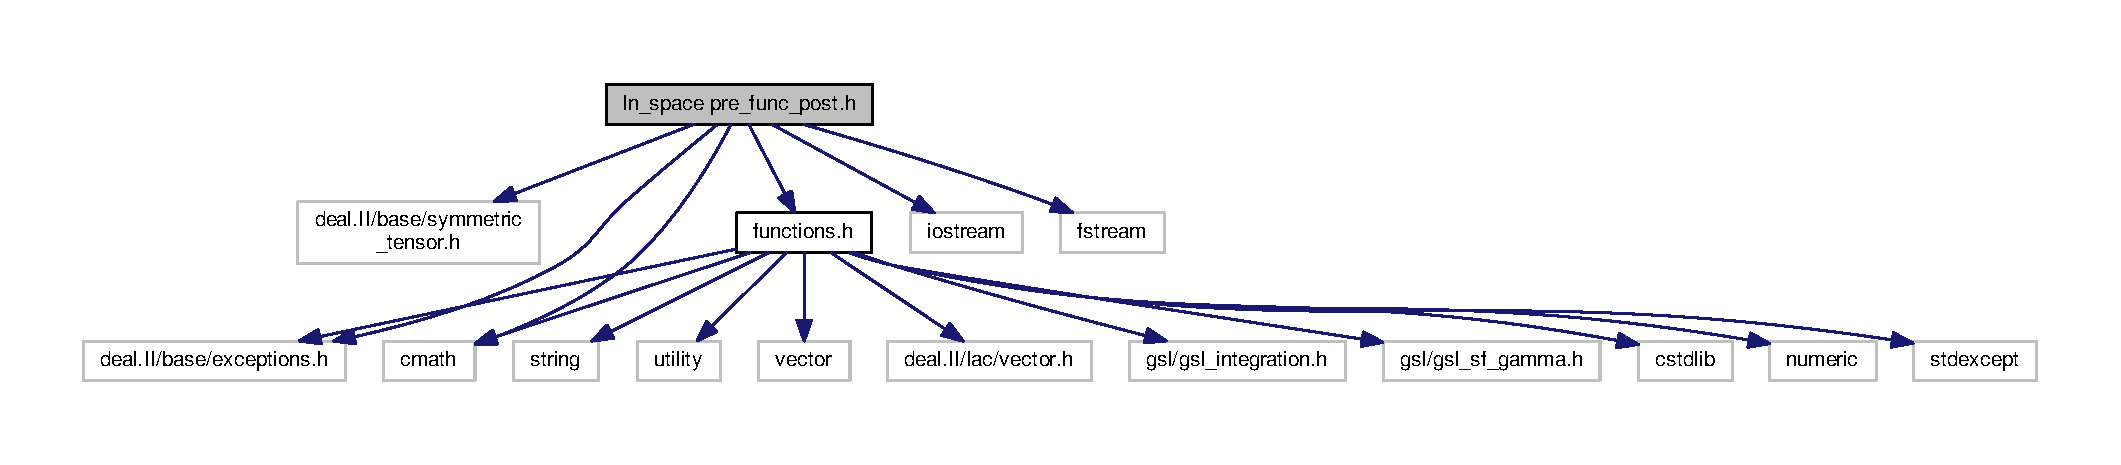
\includegraphics[width=350pt]{ln__space_01pre__func__post_8h__incl}
\end{center}
\end{figure}
\subsection*{Namespaces}
\begin{DoxyCompactItemize}
\item 
 \hyperlink{namespaceln__space}{ln\+\_\+space}
\end{DoxyCompactItemize}
\subsection*{Functions}
\begin{DoxyCompactItemize}
\item 
{\footnotesize template$<$int dim$>$ }\\void \hyperlink{namespaceln__space_a85e361462746b126386ad7e1d608e7d8}{ln\+\_\+space\+::pre\+\_\+ln} (Tensor$<$ 2, dim $>$ \&F, Symmetric\+Tensor$<$ 2, dim $>$ \&hencky\+\_\+strain, Vector$<$ double $>$ \&ea, Vector$<$ double $>$ \&da, Vector$<$ double $>$ \&fa, std\+::vector$<$ Tensor$<$ 1, dim $>$ $>$ \&eigenvector, Vector$<$ double $>$ \&eigenvalues, std\+::vector$<$ Symmetric\+Tensor$<$ 2, dim $>$ $>$ \&eigenbasis)
\item 
{\footnotesize template$<$int dim$>$ }\\void \hyperlink{namespaceln__space_a0f5e3bde0b1ee47f3dbc5977b4653342}{ln\+\_\+space\+::post\+\_\+ln} (Vector$<$ double $>$ \&ea, Vector$<$ double $>$ \&da, Vector$<$ double $>$ \&fa, Vector$<$ double $>$ \&eigenvalues, std\+::vector$<$ Symmetric\+Tensor$<$ 2, dim $>$ $>$ \&eigenbasis, Symmetric\+Tensor$<$ 2, dim $>$ \&second\+\_\+piola\+\_\+stress\+\_\+S, Symmetric\+Tensor$<$ 4, dim $>$ \&elasto\+\_\+plastic\+\_\+tangent)
\end{DoxyCompactItemize}

\hypertarget{ln__space_8h}{}\section{ln\+\_\+space.\+h File Reference}
\label{ln__space_8h}\index{ln\+\_\+space.\+h@{ln\+\_\+space.\+h}}
{\ttfamily \#include $<$deal.\+I\+I/base/symmetric\+\_\+tensor.\+h$>$}\\*
{\ttfamily \#include $<$deal.\+I\+I/base/exceptions.\+h$>$}\\*
{\ttfamily \#include $<$iostream$>$}\\*
{\ttfamily \#include $<$fstream$>$}\\*
{\ttfamily \#include $<$cmath$>$}\\*
{\ttfamily \#include \char`\"{}functions.\+h\char`\"{}}\\*
Include dependency graph for ln\+\_\+space.\+h\+:\nopagebreak
\begin{figure}[H]
\begin{center}
\leavevmode
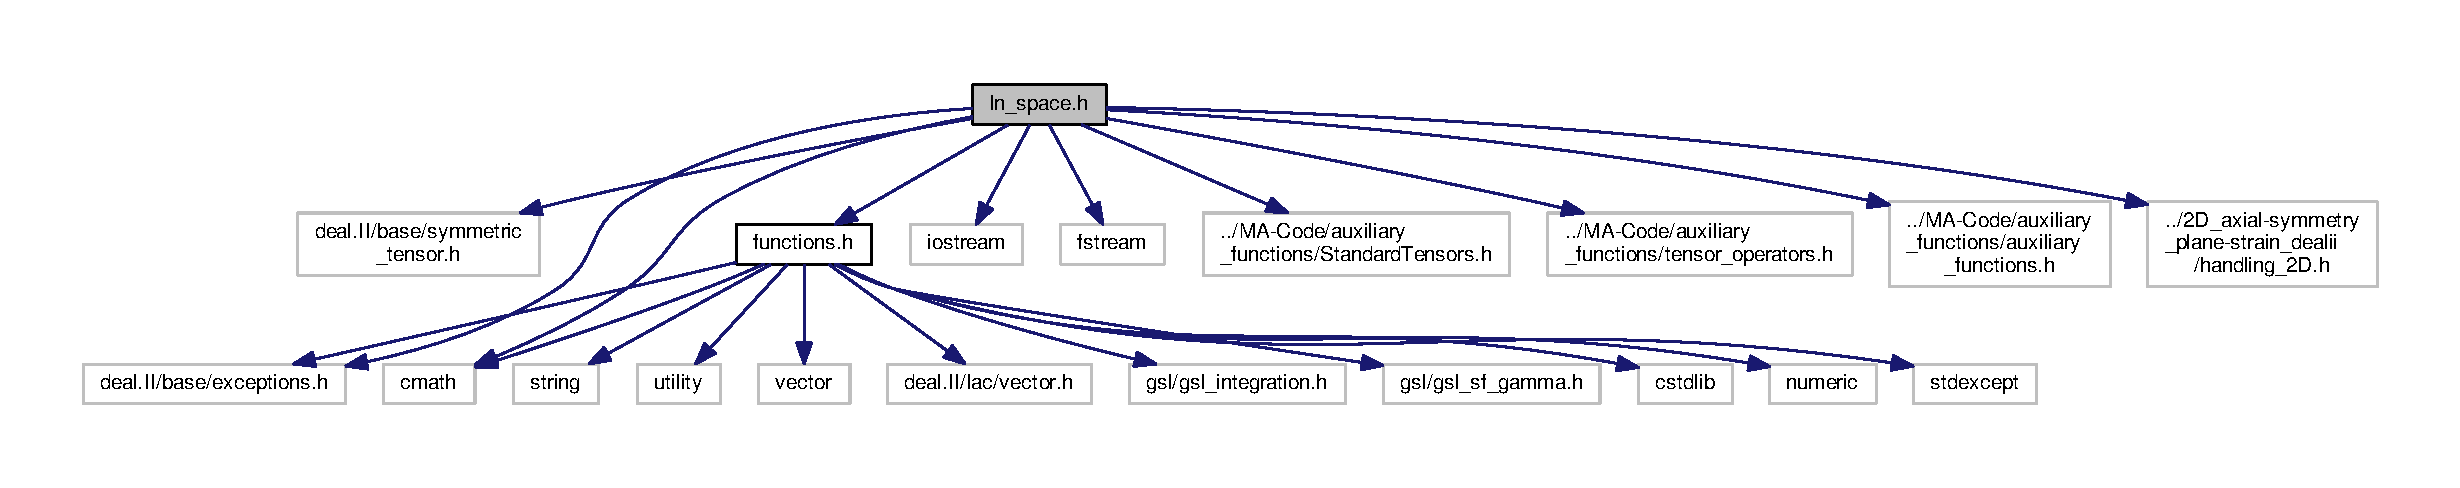
\includegraphics[width=350pt]{ln__space_8h__incl}
\end{center}
\end{figure}
\subsection*{Namespaces}
\begin{DoxyCompactItemize}
\item 
 \hyperlink{namespaceln__space}{ln\+\_\+space}
\end{DoxyCompactItemize}
\subsection*{Functions}
\begin{DoxyCompactItemize}
\item 
{\footnotesize template$<$int dim$>$ }\\void \hyperlink{namespaceln__space_a85e361462746b126386ad7e1d608e7d8}{ln\+\_\+space\+::pre\+\_\+ln} (Tensor$<$ 2, dim $>$ \&F, Symmetric\+Tensor$<$ 2, dim $>$ \&hencky\+\_\+strain, Vector$<$ double $>$ \&ea, Vector$<$ double $>$ \&da, Vector$<$ double $>$ \&fa, std\+::vector$<$ Tensor$<$ 1, dim $>$ $>$ \&eigenvector, Vector$<$ double $>$ \&eigenvalues, std\+::vector$<$ Symmetric\+Tensor$<$ 2, dim $>$ $>$ \&eigenbasis)
\item 
{\footnotesize template$<$int dim$>$ }\\void \hyperlink{namespaceln__space_a0f5e3bde0b1ee47f3dbc5977b4653342}{ln\+\_\+space\+::post\+\_\+ln} (Vector$<$ double $>$ \&ea, Vector$<$ double $>$ \&da, Vector$<$ double $>$ \&fa, Vector$<$ double $>$ \&eigenvalues, std\+::vector$<$ Symmetric\+Tensor$<$ 2, dim $>$ $>$ \&eigenbasis, Symmetric\+Tensor$<$ 2, dim $>$ \&second\+\_\+piola\+\_\+stress\+\_\+S, Symmetric\+Tensor$<$ 4, dim $>$ \&elasto\+\_\+plastic\+\_\+tangent)
\end{DoxyCompactItemize}

\hypertarget{mainpage_8h}{}\section{mainpage.\+h File Reference}
\label{mainpage_8h}\index{mainpage.\+h@{mainpage.\+h}}

\hypertarget{material_8h}{}\section{material.\+h File Reference}
\label{material_8h}\index{material.\+h@{material.\+h}}
{\ttfamily \#include $<$map$>$}\\*
{\ttfamily \#include $<$vector$>$}\\*
{\ttfamily \#include $<$math.\+h$>$}\\*
{\ttfamily \#include \char`\"{}parameters/\+All\+Parameters.\+h\char`\"{}}\\*
{\ttfamily \#include $<$deal.\+I\+I/base/exceptions.\+h$>$}\\*
{\ttfamily \#include \char`\"{}constitutive\+\_\+laws/base/\+Constitutive\+\_\+\+Law.\+h\char`\"{}}\\*
{\ttfamily \#include \char`\"{}assembly/\+M\+I\+S\+C\+Functions.\+h\char`\"{}}\\*
{\ttfamily \#include \char`\"{}materials/mechanical/base/\+Mechanical\+Material.\+h\char`\"{}}\\*
{\ttfamily \#include \char`\"{}materials/mechanical/derivatives/\+Mechanical\+Material\+\_\+\+Ti\+Al6\+V4.\+h\char`\"{}}\\*
{\ttfamily \#include \char`\"{}assembly/qph/\+Point\+History\+Mechanical\+Large\+Strain\+Incremental.\+h\char`\"{}}\\*
Include dependency graph for material.\+h\+:\nopagebreak
\begin{figure}[H]
\begin{center}
\leavevmode
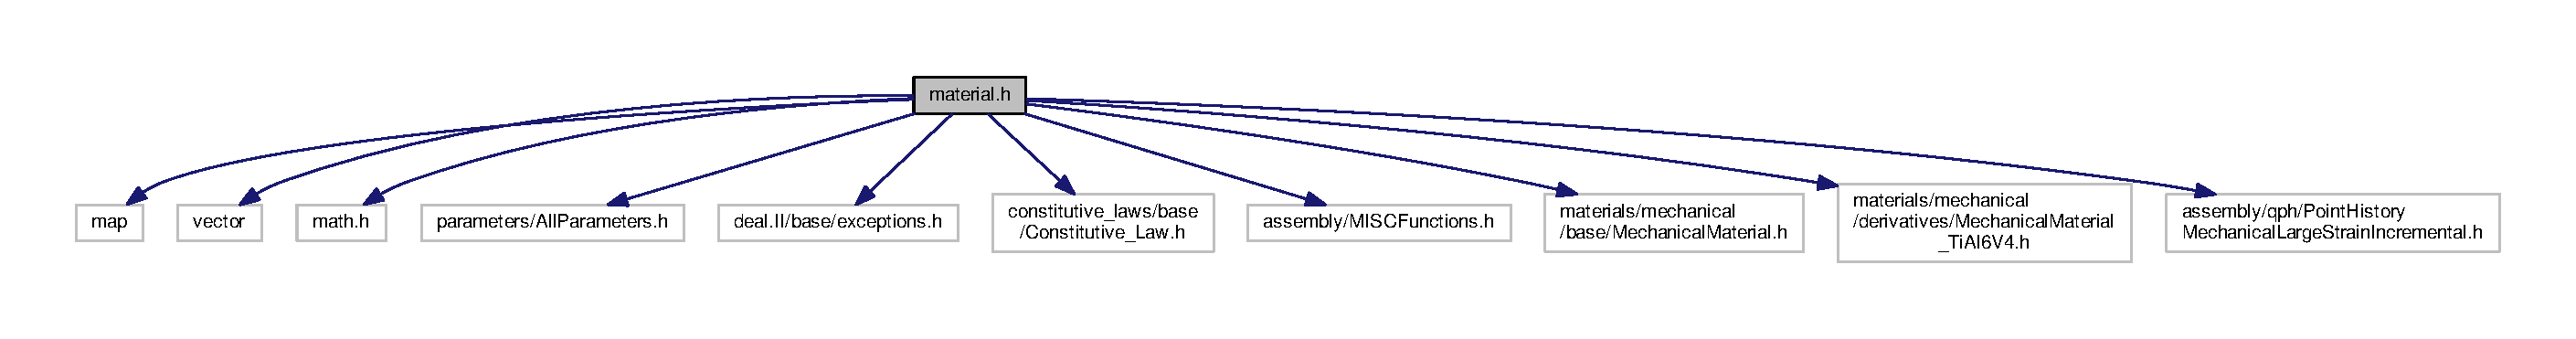
\includegraphics[width=350pt]{material_8h__incl}
\end{center}
\end{figure}
\subsection*{Classes}
\begin{DoxyCompactItemize}
\item 
class \hyperlink{classConstitutive__Laws_1_1Thermo__Elasto__Plastic}{Constitutive\+\_\+\+Laws\+::\+Thermo\+\_\+\+Elasto\+\_\+\+Plastic$<$ dim $>$}
\end{DoxyCompactItemize}
\subsection*{Namespaces}
\begin{DoxyCompactItemize}
\item 
 \hyperlink{namespaceConstitutive__Laws}{Constitutive\+\_\+\+Laws}
\end{DoxyCompactItemize}
\subsection*{Macros}
\begin{DoxyCompactItemize}
\item 
\#define \hyperlink{material_8h_afcca4bbf119fffbe56eba8681a0204e5}{C\+O\+N\+S\+T\+I\+T\+U\+T\+I\+V\+E\+\_\+\+L\+A\+W\+\_\+\+\_\+\+T\+H\+E\+R\+M\+O\+\_\+\+E\+L\+A\+S\+T\+O\+\_\+\+P\+L\+A\+S\+T\+IC}
\end{DoxyCompactItemize}


\subsection{Macro Definition Documentation}
\index{material.\+h@{material.\+h}!C\+O\+N\+S\+T\+I\+T\+U\+T\+I\+V\+E\+\_\+\+L\+A\+W\+\_\+\+\_\+\+T\+H\+E\+R\+M\+O\+\_\+\+E\+L\+A\+S\+T\+O\+\_\+\+P\+L\+A\+S\+T\+IC@{C\+O\+N\+S\+T\+I\+T\+U\+T\+I\+V\+E\+\_\+\+L\+A\+W\+\_\+\+\_\+\+T\+H\+E\+R\+M\+O\+\_\+\+E\+L\+A\+S\+T\+O\+\_\+\+P\+L\+A\+S\+T\+IC}}
\index{C\+O\+N\+S\+T\+I\+T\+U\+T\+I\+V\+E\+\_\+\+L\+A\+W\+\_\+\+\_\+\+T\+H\+E\+R\+M\+O\+\_\+\+E\+L\+A\+S\+T\+O\+\_\+\+P\+L\+A\+S\+T\+IC@{C\+O\+N\+S\+T\+I\+T\+U\+T\+I\+V\+E\+\_\+\+L\+A\+W\+\_\+\+\_\+\+T\+H\+E\+R\+M\+O\+\_\+\+E\+L\+A\+S\+T\+O\+\_\+\+P\+L\+A\+S\+T\+IC}!material.\+h@{material.\+h}}
\subsubsection[{\texorpdfstring{C\+O\+N\+S\+T\+I\+T\+U\+T\+I\+V\+E\+\_\+\+L\+A\+W\+\_\+\+\_\+\+T\+H\+E\+R\+M\+O\+\_\+\+E\+L\+A\+S\+T\+O\+\_\+\+P\+L\+A\+S\+T\+IC}{CONSTITUTIVE_LAW__THERMO_ELASTO_PLASTIC}}]{\setlength{\rightskip}{0pt plus 5cm}\#define C\+O\+N\+S\+T\+I\+T\+U\+T\+I\+V\+E\+\_\+\+L\+A\+W\+\_\+\+\_\+\+T\+H\+E\+R\+M\+O\+\_\+\+E\+L\+A\+S\+T\+O\+\_\+\+P\+L\+A\+S\+T\+IC}\hypertarget{material_8h_afcca4bbf119fffbe56eba8681a0204e5}{}\label{material_8h_afcca4bbf119fffbe56eba8681a0204e5}

%--- End generated contents ---

% Index
\backmatter
\newpage
\phantomsection
\clearemptydoublepage
\addcontentsline{toc}{chapter}{Index}
\printindex

\end{document}
